\documentclass[11pt]{article}

% Change "review" to "final" to generate the final (sometimes called camera-ready) version.
% Change to "preprint" to generate a non-anonymous version with page numbers.
\usepackage[final]{acl}

\usepackage{times}
\usepackage{latexsym}
\usepackage[T1]{fontenc}
\usepackage[utf8]{inputenc}
\usepackage{microtype}
\usepackage{inconsolata}
\usepackage{graphicx}

\usepackage{hyperref}
\usepackage{url}
\usepackage{enumitem}
\usepackage{amsmath}
\usepackage{adjustbox}
\usepackage{booktabs}
\usepackage{multirow}
\usepackage{tabularx}
\usepackage{array}
\usepackage{makecell}
% \usepackage{geometry}
\usepackage{float}
\usepackage{caption}
\usepackage{subcaption}
\usepackage{stfloats}
\usepackage{tcolorbox}

\usepackage[table, svgnames]{xcolor}
\definecolor{darkgray}{RGB}{90,90,90}
\colorlet{red}{red!50!white}
\colorlet{yellow}{yellow!50!white}
\colorlet{blue}{SkyBlue!50!white}
\colorlet{lightred}{red!90!white}
\colorlet{lightyellow}{yellow!90!white}
\colorlet{lightblue}{SkyBlue!90!white}
\colorlet{lightorange}{orange!80!white}
\colorlet{lightgreen}{LimeGreen!50!white}
\colorlet{lightpurple}{purple!40!blue!60!white}

\newcolumntype{S}{>{\raggedright\arraybackslash}m{1.46cm}}
\newcolumntype{H}{>{\raggedright\arraybackslash}m{4.09cm}}
\newcolumntype{C}{>{\centering\arraybackslash}m{0.79cm}}
\newcolumntype{M}{>{\centering\arraybackslash}m{0.68cm}}
\newcolumntype{G}{!{\color{gray!50}\vrule width 0.5pt}}
\newcommand{\grayhline}{\arrayrulecolor{gray!30}\hline\arrayrulecolor{black}}

\providecommand{\tabgain}[2]{%
#1%
\rlap{\hspace{-1.75em}\raisebox{-0.8em}{%
\tiny\textcolor{green!70!black}{#2}}}
}
\providecommand{\tabloss}[2]{%
#1%
\rlap{\hspace{-1.75em}\raisebox{-0.8em}{%
\tiny\textcolor{darkgray}{#2}}}
}
\providecommand{\tabsame}[2]{%
#1%
\rlap{\hspace{-1.75em}\raisebox{-0.8em}{%
\tiny\textcolor{darkgray}{#2}}}
}
\newcommand{\tabgainsubscript}[2]{%
  #1%
  \textsubscript{\textcolor{green!70!black}{\tiny #2}}%
}
\providecommand{\tablosssubscript}[2]{
  #1%
  \textsubscript{\textcolor{darkgray}{\tiny #2}}%
}
\providecommand{\tabsamesubscript}[2]{
  #1%
  \textsubscript{\textcolor{darkgray}{\tiny #2}}%
}

\setlength{\abovecaptionskip}{3pt}
\setlength{\belowcaptionskip}{1pt}

\renewcommand{\footnotesize}{\scriptsize}

\usepackage{silence}
\WarningFilter{latex}{Command \showhyphens has changed.}

% If the title and author information does not fit in the area allocated, uncomment the following
%
%\setlength\titlebox{<dim>}
%
% and set <dim> to something 5cm or larger.

\title{T2T-VICL: Cross-Task Visual In-Context Learning \\via Implicit Text-Driven VLMs}

% Author information can be set in various styles:
% For several authors from the same institution:
% \author{Author 1 \and ... \and Author n \\
%         Address line \\ ... \\ Address line}
% if the names do not fit well on one line use
%         Author 1 \\ {\bf Author 2} \\ ... \\ {\bf Author n} \\
% For authors from different institutions:
% \author{Author 1 \\ Address line \\  ... \\ Address line
%         \And  ... \And
%         Author n \\ Address line \\ ... \\ Address line}
% To start a separate ``row'' of authors use \AND, as in
% \author{Author 1 \\ Address line \\  ... \\ Address line
%         \AND
%         Author 2 \\ Address line \\ ... \\ Address line \And
%         Author 3 \\ Address line \\ ... \\ Address line}

% \author{Shao-Jun Xia \\
%   Duke University \\
%   \texttt{shaojun.xia@duke.edu} \\\And
%   Huixin Zhang \\
%   Texas A\&M University \\
%   \texttt{zhanghui21@tamu.edu} \\\And
%   Zhengzhong Tu \\
%   Texas A\&M University \\
%   \texttt{tzz@tamu.edu} \\
%   }

\author{
Shao-Jun Xia\thanks{Equal contribution.}\\
Duke University\\
{\texttt\small shaojun.xia@duke.edu}
\\\And
Huixin Zhang\footnotemark[1]\\
Texas A\&M University\\
{\texttt\small zhanghui21@tamu.edu}
\\\And
Zhengzhong Tu\thanks{Corresponding author.}\\
Texas A\&M University\\
{\texttt\small tzz@tamu.edu}
}

%\author{
%  \textbf{First Author\textsuperscript{1}},
%  \textbf{Second Author\textsuperscript{1,2}},
%  \textbf{Third T. Author\textsuperscript{1}},
%  \textbf{Fourth Author\textsuperscript{1}},
%\\
%  \textbf{Fifth Author\textsuperscript{1,2}},
%  \textbf{Sixth Author\textsuperscript{1}},
%  \textbf{Seventh Author\textsuperscript{1}},
%  \textbf{Eighth Author \textsuperscript{1,2,3,4}},
%\\
%  \textbf{Ninth Author\textsuperscript{1}},
%  \textbf{Tenth Author\textsuperscript{1}},
%  \textbf{Eleventh E. Author\textsuperscript{1,2,3,4,5}},
%  \textbf{Twelfth Author\textsuperscript{1}},
%\\
%  \textbf{Thirteenth Author\textsuperscript{3}},
%  \textbf{Fourteenth F. Author\textsuperscript{2,4}},
%  \textbf{Fifteenth Author\textsuperscript{1}},
%  \textbf{Sixteenth Author\textsuperscript{1}},
%\\
%  \textbf{Seventeenth S. Author\textsuperscript{4,5}},
%  \textbf{Eighteenth Author\textsuperscript{3,4}},
%  \textbf{Nineteenth N. Author\textsuperscript{2,5}},
%  \textbf{Twentieth Author\textsuperscript{1}}
%\\
%\\
%  \textsuperscript{1}Affiliation 1,
%  \textsuperscript{2}Affiliation 2,
%  \textsuperscript{3}Affiliation 3,
%  \textsuperscript{4}Affiliation 4,
%  \textsuperscript{5}Affiliation 5
%\\
%  \small{
%    \textbf{Correspondence:} \href{mailto:email@domain}{email@domain}
%  }
%}

% #########
% Submissions that do not conform to the required styles, including paper size, margin width, and font size restrictions, will be rejected without review.
% #########

\begin{document}
\maketitle
\begin{abstract}
% Visual in-context learning (VICL) aims to solve a target visual task by conditioning on a few input-output demonstrations without any model training.
% Recent advances in large vision-language models (VLMs) have shown promising VICL capability when the demonstration pair and the query belong to the same task. However, this assumption is typically impractical as the available demonstration may come from a different vision task than the query, making it unclear whether the model should imitate the demonstrated transformation or infer a new one from the query.
Visual in-context learning (VICL) solves visual tasks by conditioning on a few input-output demonstrations without any model training.
Recent advances in large vision-language models (VLMs) have shown promising VICL capability when the demonstration pair and the query belong to the same vision task, but real use cases often provide mismatched examples, making it unclear whether a VLM should imitate the demonstrated transformation or infer a new one from the query.
This raises a fundamental question:
\textbf{\textit{Can VLMs perform cross-task VICL where demonstration and query differ?}} % In the paper, we study this setting and propose T2T-VICL, a collaborative prompt-transfer framework for cross-task VICL. The key idea is to convert mismatched visual demonstrations into implicit, task-agnostic textual guidance without explicitly naming the tasks.
In the paper, we study this cross-task VICL setting and propose T2T-VICL, a collaborative prompt-transfer framework, which converts mismatched visual demonstrations into implicit textual guidance without explicitly naming the tasks.
To do so, a large teacher VLM first generates structured descriptions of visual changes and task differences between task pairs, from which we construct a dataset of diverse implicit cross-task relations. We then distill this capability into a lightweight student VLM that produces content-dependent prompts from a task-A demonstration pair and a task-B query. The generated prompt is used to guide a frozen image-editing VLM, and a score-based inference strategy is introduced to rank multiple candidates.
% Experiments on 12 low-level vision tasks and 21 evaluated cross-task pairs show that T2T-VICL consistently improves task-aware alignment over fixed prompting and often also improves image fidelity, highlighting both the potential and the current limits of cross-task VICL in VLMs.
Experiments on 12 low-level vision tasks and over 20 evaluated cross-task pairs show that T2T-VICL consistently improves task-aware alignment over fixed prompting and often also improves image fidelity, revealing both the potential and limits of cross-task VICL. Our code is available on GitHub.\footnote{\url{https://github.com/ZhangHuixin1103/Task-Transfer-VICL-in-VLM}}
\end{abstract}

\section{Introduction}
\label{sec:intro}

In-context learning (ICL) allows foundation models, especially large language models (LLMs), to adapt to new tasks from only a few input-output demonstrations, without updating model parameters~\cite{min2022rethinking, dong2022survey, highmore2024context, wang2023large, sia2024does, li2025large}.
Recent progress in large vision-language models (VLMs) has extended this paradigm from language to multimodal settings, giving rise to visual in-context learning (VICL), where a model infers an image transformation directly from a small number of visual examples~\cite{bar2022visual, wang2023painter, wang2023incontext, xprompt2024universal, zhou2024visual, ma2024vision}.
Such a capability is particularly appealing for low-level vision, where one would ideally like a single frozen model to handle diverse image restoration, removal, and generation tasks by simply conditioning on demonstrations rather than retraining for each task.

However, existing VICL methods largely rely on a restrictive \emph{same-task} assumption: the demonstration pair and the query are usually drawn from the same task. In practice, this assumption is often violated. For example, a user may only have a \emph{deraining} example while the query requires \emph{dehazing}, or may provide a reflection-removal pair while the true target is shadow removal. This mismatch makes VICL fundamentally ambiguous: should the model imitate the demonstrated transformation, or infer a different one from the query itself? At the same time, many low-level tasks are not isolated~\cite{zamir2018taskonomy, pal2019tmt, achille2019task2vec, bao2019information}. They share latent relationships in terms of visual effects, such as artifact suppression, contrast recovery, color adjustment, or illumination correction. Importantly, these relationships are often easier to express in language than in raw pixels, suggesting that language may serve as a natural bridge for transferring knowledge across mismatched visual tasks~\cite{trigka2025comprehensive, shu2024visual, brooks2023instructpix2pix, potlapalli2023promptir, conde2024instructir, ke2023neural}.

These observations motivate a new question: \emph{Can VLMs perform visual in-context learning when the demonstration and the query come from different tasks?} We study this setting as \textbf{cross-task visual in-context learning}. Compared with standard VICL, cross-task VICL requires more than pattern imitation. The model must abstract the visual change encoded in the context, reason about the discrepancy between the demonstrated task and the query task, and then produce the correct target transformation without being explicitly told the task name. A fixed prompt is often insufficient for this setting, because it provides only a generic instruction while leaving the task difference unresolved. What is needed is a mechanism that converts mismatched visual demonstrations into task-aware guidance that remains compatible with frozen VLM generators.

To this end, we propose \textbf{T2T-VICL}, a collaborative teacher-student prompting framework for cross-task VICL. Our key idea is to translate the relationship between two tasks into \emph{implicit task-difference prompts} that describe visual changes in a task-agnostic manner. A large teacher VLM first generates structured implicit descriptions from cross-task image tuples, and we curate these outputs into a benchmark of cross-task text-image relations. This capability is then distilled into a lightweight student VLM, which produces content-dependent prompts from a task-$A$ demonstration pair and a task-$B$ query. The generated prompt is fed to a frozen image-editing VLM, while an automatic score-based inference strategy, combining attribution-enhanced prompting, VLM-based visual instruction scoring~\cite{ku2023viescore}, and image quality assessment (IQA) metrics~\cite{zhang2012comprehensive}, is used to rank candidate outputs. In this way, T2T-VICL provides a practical framework for probing and improving cross-task VICL without updating the final generator model.

Our contributions are three-fold:
\begin{itemize}[itemsep=-2pt, topsep=1pt]
    \item  We formulate \textbf{cross-task VICL} for low-level vision and introduce a benchmark with implicit cross-task descriptions, enabling systematic study of how VLMs generalize across mismatched visual demonstrations. 
    \item  We propose T2T-VICL, a \textbf{VLM $\rightarrow$ sVLM $\rightarrow$ VLM} teacher-student pipeline that distills implicit task-relation knowledge from a large model into a lightweight prompt generator for frozen image-editing VLMs. 
    \item  We develop a \textbf{score-based inference framework} that couples attribution-enhanced prompting, visual instruction scoring, and IQA metrics, providing an automatic way to support and evaluate cross-task VICL.
\end{itemize}

% In-context learning (ICL) enables foundation models, such as large language models (LLMs), to easily adapt to new tasks by leveraging a few input-output demonstrations without parameter updates~\cite{min2022rethinking, dong2022survey, highmore2024context, wang2023large, sia2024does, li2025large}, achieving strong zero-shot performance in similar linguistic contextual examples. 
% Recent progress in large vision-language models (VLMs) has extended this concept from language to multimodal (text and image) conditions, with works like MAE-VQGAN~\cite{bar2022visual}, Painter~\cite{wang2023painter}, Prompt Diffusion~\cite{wang2023incontext}, and X-Prompt~\cite{xprompt2024universal} showing great promise for visual in-context learning (VICL) from only a small set of visual demonstrations ~\cite{zhou2024visual, ma2024vision}.

% Intuitively, many visual problems share underlying relationships rather than existing in isolation ~\cite{zamir2018taskonomy, pal2019tmt, achille2019task2vec}. While fully supervised approaches typically learn each task independently, this paradigm is inefficient and demands large amounts of labeled data~\cite{lecun2015deep, chum2019beyond}. Task transfer learning addresses this challenge by exploiting knowledge from source tasks to accelerate and improve performance on new targets~\cite{bao2019information}. For example, the Taskonomy~\cite{zamir2018taskonomy} framework demonstrates that by computationally modeling transfer dependencies across diverse tasks, and the possibility to derive a taxonomic map that captures both direct and higher-order relationships has been proven. Such relational phenomena are hypothesized to exist in language domains as well. Viewed through the lens of language, many image-processing-oriented low-level tasks own the same prefix or suffix~\cite{trigka2025comprehensive, shu2024visual}, e.g. ``deraining'', ``denoising'', ``dehazing'', ``deblurring'', ``demoireing''. Textual descriptions of visual differences across such tasks reveal areas of overlap as well as points of divergence. In addition, textual descriptions of generation-oriented low-level tasks such as ``colorization'', ``light enhancement'', ``harmonization'', and ``style transfer'' ~\cite{bar2022visual, ke2023neural}, primarily hinge on linguistic variations in color, illumination, and contrast. This suggests that certain latent relationships may govern the transformations between them. Meantime, several studies~\cite{brooks2023instructpix2pix, potlapalli2023promptir, conde2024instructir} have demonstrated the regulatory role of language in guiding/driving visual expressions. 

% For a standard VICL inference framework (left half in Figure~\ref{fig:fig1}), a frozen vision or vision-language model accepts paired visual examples (input images and its labels) as the ``context'' along with a query image, and produces the output image for the query. Building on the above observations, we naturally raise the key question: \textit{If the visual prompt and the images to be learned come from two different tasks, can VLMs enable VICL across different tasks? }

% In this paper, we aim at providing a VLM-agnostic methodological analysis of generalization and task abstraction in cross-task scenarios, and developing an improved diagnostic framework to evaluate the capability of cross-task VICL in VLMs. Thus we propose T2T-VICL (right half in Figure~\ref{fig:fig1}), a collaborative pipeline based on multiple VLMs that enable VICL across multiple low-level cross-task pairs. We construct a novel approach that integrates implicit descriptive textural capture, gradient-based token attribution enhancement~\cite{sundararajan2017axiomatic, nguyen2025grains}, a visual instruction-guided metric~\cite{ku2023viescore}, and image quality assessment (IQA) metrics~\cite{zhang2012comprehensive}, allowing VLMs to perform cross-task in-context learning without the need for additional training and be evaluated. Our contributions can be summarized in three aspects: (1) We propose the first comprehensive multi-VLM pipeline that automatically generates implicit text prompts to distinguish two low-level vision tasks, which can be used to explore the \textbf{boundaries of cross-task VICL}. This work also introduces the \textbf{first text-image dataset} with cross-task implicit descriptions, establishing a benchmark expected to exert lasting influence within the field. (2) We design a \textbf{VLM $\rightarrow$ sVLM} and \textbf{sVLM $\rightarrow$ VLM} framework that gets knowledge from a large-scale model into a lightweight model and leverages the compact model to get the text prompt. (3) By coupling score-based reasoning, we establish an automatic inference framework that supports cross-task VICL in VLMs while \textbf{eliminating the need for further training}.

\section{Related Work}
\label{sec:relat}

\subsection{Vision Foundation Model}
% \noindent Vision foundation models aim to unify diverse visual tasks within a single framework. Early sequence-to-sequence approaches, such as Pix2Seq~\cite{chen2022unified}, Unified-IO~\cite{lu2022unifiedio}, and OFA~\cite{wang2022ofa}, reformulated vision problems as sequence prediction and instruction-based learning. Later methods, including UViM~\cite{zhang2022uvim} and Uni-Perceiver~\cite{zhu2022uniperceiver}, introduced task-agnostic interfaces for multimodal understanding. Recent advances leverage stronger backbones and generative paradigms, e.g. Florence-2~\cite{xiao2023florence2}, InstructCV~\cite{gan2023instructcv}, and InstructDiffusion~\cite{geng2023instructdiffusion}, enabling prompt-driven recognition and conditional generation under a unified architecture.

% Most notably, VLMs have emerged as unified frameworks that couple visual encoders with large language models under instruction-driven settings. Emu ~\cite{sun2023emu, wang2024emu3} series integrate diffusion models with LLM-predicted embeddings, functioning as a generalist model capable of handling diverse vision tasks. Chameleon~\cite{chameleon2024} team follows an early-fusion strategy, integrating text and image tokens from the outset to support interleaved understanding and generation. In contrast, Transfusion~\cite{transfusion2024} combines next-token prediction for language with diffusion for images, and Show-o~\cite{showo2024} extends this hybrid approach with a one-transformer design that merges auto-regression and discrete diffusion. Collectively, these efforts highlight the trend of VLMs shaping the evolution of vision generalist models.

\noindent Vision foundation models aim to unify diverse visual tasks within a single framework. Early approaches reformulated vision problems as sequence prediction or instruction-based learning (Pix2Seq~\cite{chen2022unified}, Unified-IO~\cite{lu2022unifiedio}, OFA~\cite{wang2022ofa}), while later works introduced task-agnostic multimodal interfaces (UViM~\cite{zhang2022uvim}, Uni-Perceiver~\cite{zhu2022uniperceiver}). Recent advances further leverage stronger multimodal backbones and instruction-driven paradigms for prompt-based recognition and conditional generation (Florence-2~\cite{xiao2023florence2}, InstructCV~\cite{gan2023instructcv}, InstructDiffusion~\cite{geng2023instructdiffusion}). Meanwhile, VLMs have emerged as powerful vision generalists through unified multimodal architectures, including Emu~\cite{sun2023emu,wang2024emu3}, Chameleon~\cite{chameleon2024}, Transfusion~\cite{transfusion2024}, and Show-o~\cite{showo2024}. Collectively, these efforts highlight the trend of VLMs shaping the evolution of vision generalist models.

\subsection{Visual In-Context Learning}
Visual in-context learning (VICL) refers to adapting vision models to downstream tasks through contextual examples rather than explicit fine-tuning, and it can be broadly divided into visual prompting and prompt-driven conditioning. Implicit prompting methods, represented by MAE-VQGAN~\cite{bar2022visual} and Painter~\cite{wang2023painter}, rely on masked prediction or image completion as objectives, enabling models to generalize under diverse vision tasks. In contrast, explicit prompt-driven approaches leverage explicit conditioning to adapt diverse vision problems. For instance, Prompt Diffusion~\cite{wang2023incontext} exploits diffusion-based generation under prompt guidance. While PromptGIP~\cite{liu2023promptgip} adopts QA-style prompt structures. Additional works such as CoOp~\cite{zhou2022coop} and VPT ~\cite{jia2022vpt} further extend VICL by introducing learnable prompts for vision transformers. More recently, X-Prompt~\cite{xprompt2024universal} targets general image generation, compressing contextual signals and unifying diverse vision tasks within an auto-regressive framework. Most existing VICL methods focus on performing the visual prompt and query image in the same tasks, our T2T-VICL extends this paradigm to difficult cross-task settings, where the visual prompt and query image are from different tasks, digging the potential knowledge adaptation across diverse vision tasks.

\begin{figure*}[ht]
    \centering
    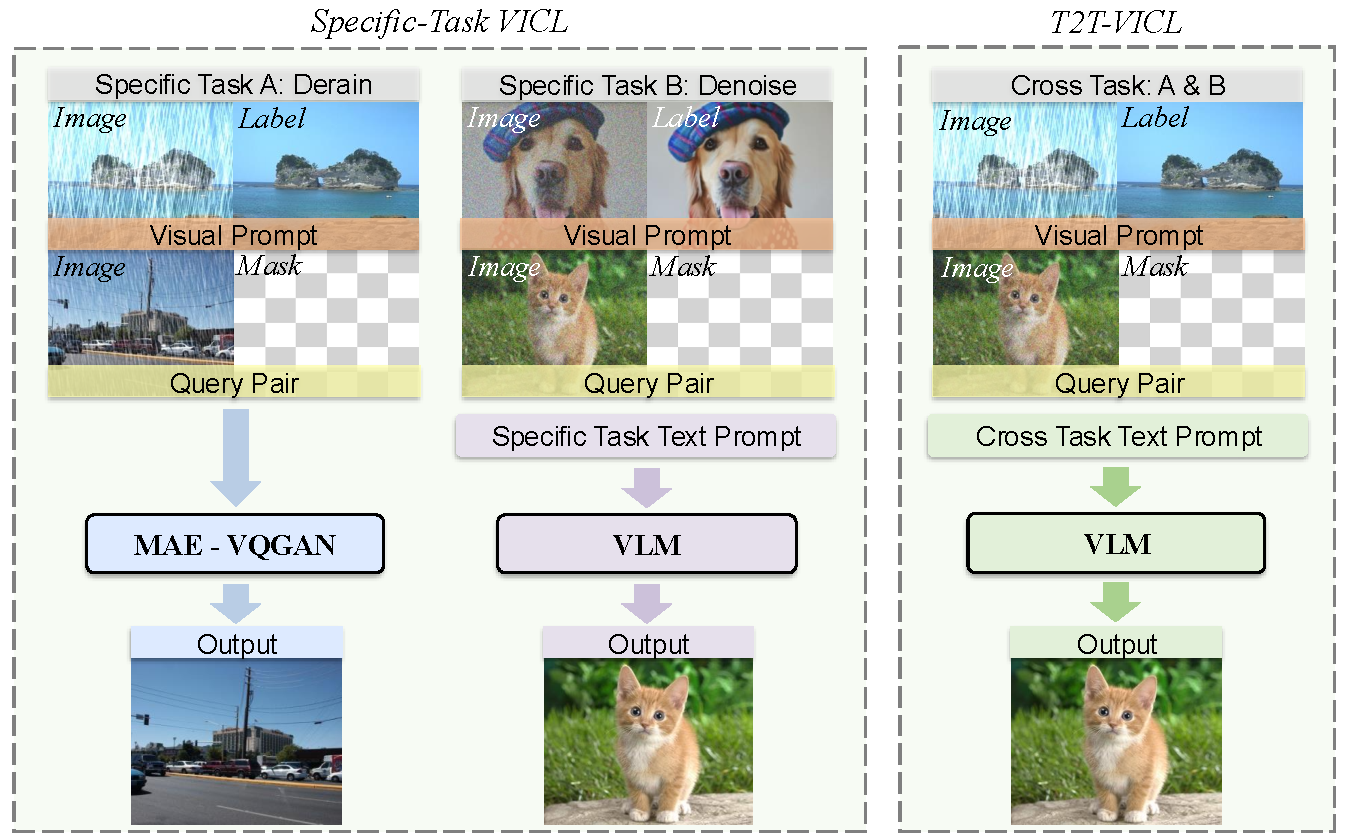
\includegraphics[width=0.9\textwidth]{fig/figure1vertical.pdf}
    \caption{Illustration of Cross-Task Visual In-Context Learning}
    \label{fig:fig1}
\vspace{-8pt}
\end{figure*}

\subsection{Task Transfer}
Task generalization refers to leveraging knowledge from previously solved tasks to facilitate learning on unseen ones. Early milestones such as Taskonomy ~\cite{zamir2018taskonomy} provided the first large-scale analysis of transferability across 26 vision tasks, introducing the task affinity matrix as a foundation for cross-task generalization. Following this line, TMT~\cite{pal2019tmt} extended Taskonomy by applying matrix factorization to refine the estimation of inter-task transferability. Similarly, Task2Vec~\cite{achille2019task2vec} proposed embedding tasks into a vector space using Fisher information, making task similarity measurable and interpretable. Beyond these foundations,~\cite{standley2020mtl} systematically investigated which tasks should be learned together in multitask settings, highlighting task affinity as a guiding principle. Paper~\cite {dwivedi2019crosstask} introduced cross-task consistency to enforce relational constraints. Given the growing visual generation ability of VLMs, the progress in this field motivates our exploration of cross-task generalization in VLMs and unlocks the boundaries.

\subsection{Language-Driven Image Editing}
\noindent Language-driven vision restoration has evolved from instruction-guided editing to adaptive prompt-based restoration. Early works such as InstructPix2Pix~\cite{brooks2023instructpix2pix}, InstructIR~\cite{conde2024instructir}, and PromptIR~\cite{potlapalli2023promptir} showed that natural language can guide fine-grained, degradation-aware manipulation of image features. Subsequent studies including SPIRE~\cite{qi2024spire}, PromptFix~\cite{yu2024promptfix}, Perceive-IR~\cite{zhang2025perceive}, and FPro~\cite{zhou2024fpro} further enriched semantic and perceptual prompting, enabling finer control over fidelity and restoration strength. These advances establish natural language as a direct and interpretable driver for low-level vision tasks.

\section{Framework}
\label{sec:method}

\begin{figure*}[t]
    \centering
    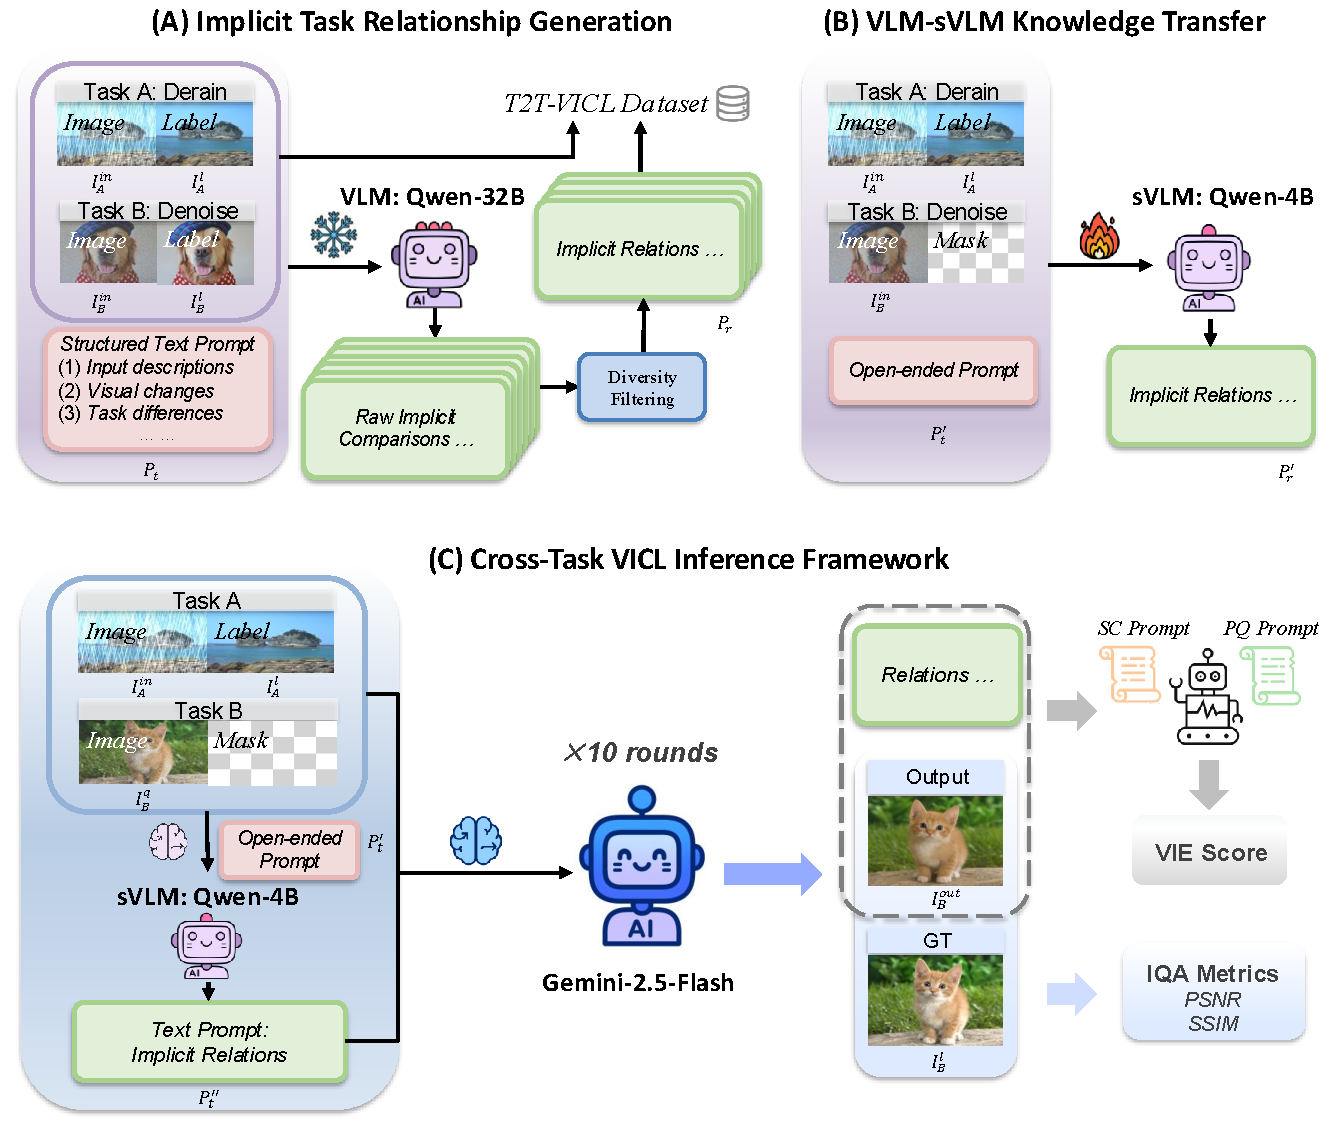
\includegraphics[width=0.88\textwidth]{fig/figure2simple.pdf}
    \caption{Overview of the Proposed Pipeline and its Workflow}
    \label{fig:fig2}
\vspace{-8pt}
\end{figure*}

\subsection{T2T-VICL: Overview of VLM Pipeline}
To explore the boundaries of cross-Task VICL via VLMs, we propose T2T-VICL, a collaborative pipeline that leverages the complementary strengths of large and small language VLMs to enhance vision-language reasoning. First, a large pre-trained VLM generates implicit textual descriptions for two distinct tasks, while the linguistic reliability of these descriptions is quantitatively evaluated. To enable efficient deployment, we fine-tune a sVLM to transfer the reasoning capabilities of the large model while reducing computational overhead. During inference, the sVLM produces text prompts to the final large VLM, thereby guiding the downstream reasoning process. Our main VLM inference pipeline aligns with the standard VICL setting, while the trained sVLM is only an auxiliary component which extracts implicit task descriptions from visual examples and generates text prompts without altering the main inference branch. Finally, candidate results are ranked by another VLM with a visual instruction-guided metric and IQA metrics, and the optimal outcome is selected from the top-k candidates.

\subsection{Implicit Relationship Generation}
We begin by automatically generating rich textual descriptions that implicitly capture the differences between two low-level vision tasks. We consider 12 diverse low-level tasks into three categories as Table~\ref{tab:1}, spanning classic degradation problems (deraining, dehazing, denoising, deblurring, demoireing), removal tasks (shadow removal, reflection removal) as well as generation/enhancement tasks (colorization, low-light enhancement, harmonization, inpainting, style transfer). For any arbitrary pair of tasks A and B, our goal is to obtain an implicit text prompt that depicts the difference without explicitly naming either task. To accomplish this, we leverage large vision-language model Qwen2.5-VL-32B-Instruct, which takes two image pairs as input. We design the text prompt $P_t$ to provide structured comparisons of two tasks: (1) image descriptions---the basic content of the figures from task A and B; (2) visual changes---observable image-level changes, as opposed to labels for each task; and (3) task differences---the perceptible improvements or modifications after applying the task. Crucially, the prompt instructs the VLM to compare these aspects for task A versus task B without explicitly pushing the model to know the task name (not tell the model what exactly the tasks should do), ensuring the description is extremely implicit. This mechanism forces the VLM to articulate the subtle differences in a narrative manner. Meanwhile, we also consider the baseline setting, where the VLM performs VICL with a fixed prompt. Details of the implicit and fixed prompts are provided in Appendix Sec.~\ref{sec:prompt}.

% \begin{table}[h!]
% \centering
% \caption{Categorization of Low-Level Vision Tasks}
% \begin{tabular}{p{2.5cm} p{5.5cm}}
% \hline
% \textbf{Category} & \textbf{Tasks} \\ \hline
% \textbf{Restoration} & Deblurring, Dehazing, Denoising, Deraining, Demoireing \\[3pt]
% \textbf{Removal} & Reflection Removal, Shadow Removal \\[3pt]
% \textbf{Generation / Enhancement} & Style Transfer, Light Enhancement, Colorization, Harmonization \\ \hline
% \end{tabular}
% \label{tab:task_categories}
% \end{table}

% \begin{table}[h!]
% \centering
% \caption{Categorization of Low-Level Vision Tasks}
% \begin{tabular}{p{2.8cm} p{5.4cm}}
% \hline
% \textbf{Category} & \textbf{Tasks} \\ \hline
% \textbf{Restoration} & Deblurring, Dehazing, Denoising, Deraining, Demoireing \\[3pt]
% \textbf{Removal} & Reflection Removal, Shadow Removal \\[3pt]
% \textbf{Generation / Enhancement} & Style Transfer, Light Enhancement, Colorization, Harmonization \\[3pt]
% \textbf{Cross-Task Combination} & Inter-category compositions such as   Deblurring $\rightarrow$ Demoireing or Intra-category compositions such as Reflection Removal $\rightarrow$ Dehazing \\ \hline
% \end{tabular}
% \label{tab:task_categories}
% \end{table}

\begin{table}[!ht]
\vspace{-6pt}
\centering
\footnotesize
\captionsetup{width=0.99\columnwidth, skip=4pt, type=table}
\caption{Categorization of low-level vision tasks. Based on this, we divide cross-task pairs into \textbf{intra-category} compositions such as ``Deblurring $\rightarrow$ Demoireing'', and \textbf{inter-category} compositions such as ``Reflection Removal $\rightarrow$ Dehazing''.}
\vspace{-1pt}
\renewcommand{\arraystretch}{1}
\begin{tabularx}{\columnwidth}{p{0.24\columnwidth} X}
\hline
\textbf{Category} & \textbf{Tasks} \\ \hline
\rowcolor{lightred!30}
\textbf{Restoration} & \makecell[l]{Deblurring, Dehazing, Demoireing, \\Denoising, Deraining} \\
\rowcolor{lightyellow!30}
\textbf{Removal} & Reflection Removal, Shadow Removal \\
\rowcolor{lightblue!30}
\textbf{Generation\slash Enhancement} & Colorization, Harmonization, Inpainting, Light Enhancement, Style Transfer \\
\hline
\end{tabularx}
\label{tab:1}
\vspace{-6pt}
\end{table}


Subsequently, the above procedure is implemented for all the included low-level tasks to build a high-quality benchmark dataset. For each pair of tasks A and B, we sampled a large number of combinations from public datasets and queried the VLM with each sample to get a text output: (i) an input image $I_A^{in}$ and its label $I_A^{l}$ from task A, and (ii) an input image $I_B^{in}$ with the label $I_B^{l}$ from different task B. Thus we obtained the implicit textural relations:
\begin{equation}
P_r = M_l(I_A^{in}, I_A^{l}, I_B^{in}, I_B^{l}, P_t),
\end{equation}
The model is trained to generate the corresponding comparison text that the teacher (32B model) had produced for that pairing. However, the VLM can sometimes produce repetitive or overly generic statements, especially if many samples share similar traits. We therefore conducted a diversity filtering method by using semantic sentence embeddings. We encoded each candidate description with a SentenceTransformer~\cite{reimers2019sentence} (all-MiniLM-L6-v2) to obtain a dense vector representation. This allowed us to quantitatively measure similarities among the descriptions. We then performed clustering in embedding space to detect groups of near-duplicates or redundant phrasing. In this manner, we filtered out repetitive outputs and retained only one representative with the most distinct descriptions. Ultimately, we kept 2,000 diverse descriptions per task pair. To our knowledge, this is the first text-and-image dataset that implicitly captures cross-task relationships, providing the foundation for our next steps.


%\textcolor{blue}{
%\textbf{Datasets and tasks.} We curate twelve low-level vision tasks with canonical sources widely adopted in prior work \textcolor{red}{Add ref}: deblurring (GOPRO), dehazing (D-HAZY), demoireing (UHDM), denoising (SIDD), deraining (RainCityscapes), harmonization (iHarmony4), inpainting (modified DIV2K), colorization (modified DIV2K), low-light enhancement (LoL), reflection removal (SIR$^2$), shadow removal (ISTD), and style transfer (Night2Day). This mix spans degradations (blur, haze, noise, weather streaks, reflections, shadows) and generative transformations (recoloring, illumination/style changes), giving broad coverage for cross-task comparisons used in our framework.}

%\textcolor{blue}{
%\textbf{VLM-as-analyst protocol.} We employ Qwen2.5-VL-32B-Instruct as a descriptive oracle that receives two task exemplars—typically an input→output pair from task A and an input→output pair from task B—together with a structured comparative prompt. The model is instructed to articulate, for each task: (i) the target goal (what the transformation achieves), (ii) the input degradation (artifact type), and (iii) the perceptual changes from input to output. This forces the VLM to reason about abstract phenomena (e.g., global haze veil vs. localized rain streaks, loss of sharpness vs. sensor noise) rather than only recognizing objects. In a practical variant used during data conversion, we sometimes reveal only B's input (no B output) and explicitly ask the model to infer B's transformation type—encouraging robustness to partially observed task pairs.}

%\textcolor{blue}{
%\textbf{Scaling and filtering.} For every ordered task pair, we sample many image examples and query the oracle repeatedly to obtain 2000+ comparative narratives. Because raw generations may be redundant, we embed each description using SentenceTransformer (all-MiniLM-L6-v2), cluster in embedding space, and retain diverse, informative representatives (unused images are reserved for final inference). The result is a curated text corpus that externalizes inter-task relations in natural language.}

%\textcolor{blue}{
%\textbf{Positioning to prior art.} Earlier approaches quantify task affinity with embeddings or transfer matrices (e.g., Task2Vec: Task Embedding for Meta-Learning [https://arxiv.org/abs/1902.03545]; Taskonomy: Disentangling Task Transfer Learning [https://arxiv.org/abs/1804.08328]), which are effective but opaque. Concurrently, language has been used to control restoration models via prompts or instructions (PromptIR: Prompting for All-in-One Blind Image Restoration [https://openreview.net/forum?id=KAlSIL4tXU]; InstructIR: High-Quality Image Restoration Following Human Instructions [https://arxiv.org/abs/2401.16468]; Perceive-IR: Learning to Perceive Degradation Better for All-in-One Image Restoration [https://arxiv.org/abs/2408.15994]). Our contribution is complementary: we use a large VLM to produce textual explanations that act as human-interpretable supervision for cross-task reasoning, rather than as mere control signals. These narratives constitute a language-guided, interpretable proxy for task affinity that we subsequently transfer to a compact model.}


%Traditional task transfer frameworks often quantify inter-task similarity through performance gains or learned embeddings – for example, Taskonomy's transfer matrix or vectorial task embeddings like Task2Vec (Task2Vec: Task Embedding for Meta-Learning [https://arxiv.org/abs/1902.03545]). While such metrics yield a coarse quantitative affinity between tasks, they offer little in terms of human intuition or why certain tasks relate. In this work, we pivot to a qualitatively rich, language-centric approach: we leverage a large vision-language model (VLM) to automatically describe the differences between low-level vision tasks in natural language. By casting task relationships into descriptive text, we obtain a human-interpretable ``affinity measure'' that complements numeric metrics. This idea is inspired by emerging evidence that natural language can act as a powerful driver for fine-grained visual reasoning in VLMs (e.g. instructing image edits or transformations) – turning what was once an implicit relationship into an explicit narrative that can guide learning.

%We evaluate our approach on a curated benchmark of twelve low-level vision tasks, each paired with a standard dataset from prior literature. The selection covers a broad spectrum of image enhancement and transformation problems, ensuring that we include both traditional restoration tasks and more creative alterations. On the restoration side, our tasks include image deblurring (using the GoPro dataset for motion blur removal), image denoising (using SIDD for sensor noise reduction), single-image deraining (RainCityscapes dataset, focusing on removing rain streaks), image dehazing (D-HAZY, for eliminating atmospheric haze), demoireing (UHDM dataset to remove moiré patterns), reflection removal (SIR$^2$ for eliminating glass/window reflections), shadow removal (ISTD benchmark for removing cast shadows), and low-light enhancement (LoL dataset for brightening dark images). In addition, we include tasks that involve more generative or recoloring transformations: image colorization (using a custom dataset derived from DIV2K, where grayscale images are colorized), image inpainting (also based on modified DIV2K, filling in missing or masked-out regions), image harmonization (iHarmony4 dataset, adjusting the appearance of a composite image to make pasted objects blend naturally), and style transfer (Night2Day, a task that transforms nighttime scenes to daytime style). Together, these 12 tasks and their datasets form the foundation of our experiments. They provide a diverse testbed for generating cross-task prompts – for any given pair of tasks, we draw on these datasets to supply example input/output pairs. The variety of content (from natural outdoor scenes in RainCityscapes to specific artifacts in UHDM) and the mix of degradation types ensure that our model learns to describe a wide range of differences. By using established datasets, we also ensure that our results are comparable to prior works and grounded in realistic image conditions rather than synthetic toy data. This rich benchmark enables us to thoroughly explore how visual in-context learning can be achieved across many distinct low-level vision challenges.

%Concretely, we use the 32B-parameter Qwen2.5-VL-32B-Instruct model as a descriptive oracle to generate comparative narratives for pairs of tasks. Each query to the oracle consists of two image pairs: one input-output example from task A and one input-output example from task B. We prompt the VLM to behave like an expert analyst, systematically comparing the two tasks. The prompt is structured to elicit three key pieces of information for each task: (1) the target goal – what the task's output is meant to achieve (e.g. ``remove rain streaks'' or ``sharpen blurred details''); (2) the input degradation – the type of distortion or artifact present in the task's input image (rain, haze, blur, noise, etc.); and (3) the visual changes from input to output – what perceptible improvements or alterations occur after applying the task. By explicitly requesting these details for both tasks, the model is forced to articulate the subtle differences in what each task does and how it affects the image. For example, given a deraining input-output pair versus a dehazing pair, the oracle might respond with a multi-sentence explanation detailing how Task A targets removing rain streaks and restoring clear backgrounds (addressing water droplets as the degradation), whereas Task B aims to eliminate distant fog to recover contrast (with haze as the degradation), and it would highlight distinct visual improvements achieved by each. This multi-part comparative prompting ensures a granular analysis of each task in parallel, pushing the VLM beyond object recognition into reasoning about abstract visual concepts like ``blurriness,'' ``color cast,'' or ``shadow softness'' and how each is remedied.

%The textual outputs from this process serve as an implicit task relationship measure in a human-readable form. Instead of a single similarity score or latent vector, we obtain a nuanced linguistic depiction of how two tasks relate and differ. This approach externalizes the model's internal reasoning into natural language, which is far more interpretable to humans (and potentially to other models) than opaque embeddings. In essence, the large VLM is distilling its cross-task understanding into text. These descriptive comparisons can reveal, for instance, that deblurring and denoising both focus on removing high-frequency artifacts (blur vs. noise) but differ in the visual patterns they target, or that colorization and inpainting are more dissimilar because one hallucinates plausible colors for a grayscale image while the other fills in missing regions with context-appropriate content. Such insights go well beyond what a Task2Vec vector or cosine similarity might convey, highlighting why tasks cluster together. We consider this a form of language-guided task affinity, where relationships are captured by semantic narratives rather than just numbers. This idea builds on prior explorations of using language to guide vision tasks – for example, recent works have shown that language prompts can control image restoration models (PromptIR: Prompting for All-in-One Blind Image Restoration [https://openreview.net/forum?id=KAlSIL4tXU]) or that human instructions enable flexible image enhancements (InstructIR: High-Quality Image Restoration Following Human Instructions [https://arxiv.org/abs/2401.16468]). However, those methods use language as input for a single model's operation. In contrast, our framework uses language as an intermediary output: the VLM's own descriptions become a tool for analyzing and eventually improving multi-task learning. This novel use of descriptions as supervision differentiates our work from prior ``language-driven restoration'' efforts like InstructIR, PromptIR, or Perceive-IR (Perceive-IR: Learning to Perceive Degradation Better for All-in-One Image Restoration [https://arxiv.org/abs/2408.15994]), which primarily integrate text to direct the restoration process. Here, text is elevated to a first-class representation of task knowledge.

%To build a high-quality dataset of these implicit task relationship descriptions, we systematically generated comparisons for all pairs of tasks in our benchmark. We curated 12 diverse low-level vision tasks (detailed in the Dataset Description below), covering both standard degradation-removal tasks and more generative image transformations. For each ordered pair of tasks (A vs B), we sampled a large set of image examples from their respective datasets. Each sample consisted of one input-output pair from task A and one from task B, which we then fed into Qwen2.5-VL-32B with the standardized comparative prompt. We repeated this process to accumulate over 2,000 raw descriptions per task pair, ensuring broad coverage of different image content and conditions. The result was a substantial corpus of model-generated task comparisons – on the order of tens of thousands of descriptions overall. Qualitatively, we found that the VLM's responses often captured insightful distinctions (e.g. noting that deraining needs to handle occluding streaks on surfaces, whereas dehazing deals with a global veil that washes out distant objects). The use of such a powerful VLM was crucial: a smaller model might miss these subtleties or fall into trivial statements.

%However, not every raw generation is ideal for training. The oracle sometimes produces repetitive or overly-generalized text, especially when many images share similar traits. To address this, we implemented a filtering and selection pipeline using semantic embeddings. We encoded each candidate description using a SentenceTransformer model (all-MiniLM-L6-v2), which maps the sentence(s) into a dense vector embedding. This allowed us to measure the pairwise similarity between descriptions quantitatively. Our goal was to retain the most diverse and informative descriptions from the 2,000+ outputs per pair. We performed clustering in the embedding space to identify groups of very similar descriptions – for instance, several outputs might all say essentially ``Task A clears blur while Task B clears haze'' with minor wording differences. From each cluster, we kept one representative description and discarded redundancies. In this manner, we distilled the corpus down to a curated subset of highly distinct narratives. Ultimately, we kept roughly 2,000 descriptions per task pair (i.e. filtering out a large portion of duplicates and less useful outputs), though the exact number varied with the complexity of the pair. This curation process ensures that the final training data covers a wide range of observations: from common high-level comparisons to niche insights that appeared only in a few examples. By constructing this filtered text dataset, we effectively created a new resource – a text-and-image corpus that implicitly captures cross-task relationships. Such a dataset is, to our knowledge, the first of its kind, and it provides the foundation for the next stage of our pipeline: using these descriptions to transfer knowledge into a smaller model.

\subsection{VLM-sVLM Knowledge Transfer}

\subsubsection{Large-to-Small Transfer Framework}

% \textbf{Knowledge transfer and teacher-student model construction.}
Having obtained the implicit task comparisons from the large VLM, we next transfer this knowledge into a Qwen3-VL-4B-Instruct model as a student. By using the generated text prompts in section 3.2 as targets, we fine-tuned the student model with three input images $I_A^{in}$, $I_A^{l}$, and $I_B^{in}$. Differently, we omit the label of task B $I_B^{l}$ here. By using an open-ended prompt $P_t^{'}$ (e.g. ``Compare the observed in these images''), we force the 4B model to learn the effect of task B solely from the characteristics of input and output the implicit textural relations $P_r^{'}$.
\begin{equation}
P_r' = M_s(I_A^{in}, I_A^{l}, I_B^{in}, P_t'),
\end{equation}
We format each training instance in the official Qwen-VL conversational style, which includes a system instruction and the images embedded with markdown tags. The student is then trained to produce the teacher's full comparison text as the completion. The training objective is to minimize the cross-entropy loss between the generated text from the student and the reference description from the teacher. Through many epochs of exposure to different task pairs and images, the sVLM model gradually learns the ``reasoning habit'' from the teacher model and becomes capable of producing these comparisons on its own. In effect, the implicit knowledge of inter-task relationships is transferred into the small model at the language level.

% \noindent \textbf{Model choice and training efficiency.}
We selected Qwen3-VL-4B as the student not only for its manageable size, but also because it shares the same architecture and multimodal interfaces as the teacher model. After training, the fine-tuned 4B model is indeed able to take two image pairs from tasks A and B and directly output a coherent comparison of the tasks, much like the 32B model did. In other words, the student has learned to be a ``narrative engine'' that explains cross-task relationships on demand. This approach is related in spirit to recent prompt-based tuning methods in vision-language models~\cite{zhou2022coop}. But the key difference is that instead of learning a static prompt vector or fixed set of words for a model, we train a full generative model to produce dynamic, content-dependent prompts. The student can flexibly generate different comparative descriptions for different image pairs, rather than a single fixed prompt. By using the outputs of the large model as textual supervision, we effectively compress its high-level reasoning about tasks into a lightweight model.


\subsubsection{Small-to-Large Deployment Framework}

Once the student model is trained, we deploy it as a front-end module to assist the large model during inference and provide the text prompt, which is then consumed by the larger VLM for final reasoning and output image generation. This hierarchical approach reduces reliance on heavy computation during the initial stages of inference while preserving the representational capacity of large-scale VLMs. This is essentially a reverse direction of knowledge flow---the Small $\rightarrow$ Large step uses the student model to guide the final inference model (Gemini-2.5-flash). The process employs the trained Qwen3-VL-4B model to process the input of the visual prompt ($I_A^{in}$, $I_A^{l}$), query image $I_B^{q}$ and text prompt $P_t'$, output a prompt representation $P_t''$ as following:
\begin{equation}
P_t'' = M_s(I_A^{in}, I_A^l, I_B^q, P_t').
\end{equation}
By offloading this initial abstraction to $M_s$, we reduce the computational 
overhead associated with feeding raw multimodal inputs directly into the large model.

The generated prompt $P_t''$ is then provided as an input to a larger VLM $M_\ell$, which possesses stronger representational power and reasoning ability. Specifically, 
\begin{equation}
I_B^{out} = M_\ell(I_A^{in}, I_A^l, I_B^q, P_t''),
\end{equation}
where $I_B^{out}$ denotes the model prediction, and this step enables $M_\ell$ to focus on higher-level reasoning. The large VLM can focus on executing the described transformation on the query image, rather than figuring out from scratch what the transformation should be. More importantly, this two-stage deployment is highly interpretable: the intermediate text prompt $P_t''$ clearly explains the intended operation, providing transparency into the decision-making. It also offers a point of control that a human or another module could modify or validate the prompt before the final image generation. This loop leverages the complementary strengths of each model size, the powerful reasoning and generation of large VLM and the efficiency and fast text generation of sVLM to achieve cross-task visual in-context learning that is both effective and practical. 

%where the sign of $z_j(n)$ indicates whether token $n_j$ favors the positive or negative class. 
%Finally, the top-$k$ tokens are selected by applying a top-$k$ operator:
%\begin{equation}
%I^{+}_k(n) = \mathrm{TopK}\big(z(n), k\big), \quad
%I^{-}_k(n) = \mathrm{TopK}\big(-z(n), k\big).
%\end{equation}
%These sets provide the token-level evidence that will be used to construct steering directions in the following step.

\subsubsection{Score-Based Reasoning}

To enhance decision-making, we introduce perceptual score-based screening based on VIEScore~\cite{ku2023viescore}. Since conventional image-synthesis metrics are often task-agnostic and opaque, they provide a single number without revealing why an image is judged good or bad. In contrast, VIEScore is a task-aware and explainable evaluator driven by a VLM. Given an instruction $I$, a synthesized image $O$, and a set of conditions $C^*$, the evaluator first produces a natural-language rationale and then a scalar score $s$:
\begin{equation}
f_{\text{VIE}}(I,O,C^{*}) = (\text{rationale},\, s).
\end{equation}
To reflect the ``weakest-link'' nature of conditional generation, we decompose the score into
\emph{Semantic Consistency} (SC) and \emph{Perceptual Quality} (PQ). 
Each is formed by minimum aggregation over task-specific sub-scores $\{\alpha_i\}$ and $\{\beta_j\}$ (0--10 scale, later normalized):
\[
\mathrm{SC}=\min_i \alpha_i,\qquad \mathrm{PQ}=\min_j \beta_j.
\]
The final overall rating uses a geometric mean:
\begin{equation}
O=\big(\mathrm{SC}\cdot \mathrm{PQ}\big)^{1/2}.
\end{equation}
In practice, we prompt the VLM with explicit rubrics for SC and PQ; notably, PQ is assessed from the synthesized image alone (to avoid instruction confounds), while SC conditions are presented alongside the image. 
This design yields interpretable rationales, task-aware scores, and robust correlations with human judgments across diverse conditional image tasks.

% \begin{table*}[ht]
% \centering
% \captionsetup{width=0.78\textwidth, skip=4pt, type=table}
% \caption{Average of evaluation metrics in the top-tier group. Generated by Gemini with Qwen prompts, compared to the fixed-prompt baseline.}
% \vspace{-1pt}

% \small
% % \setlength{\tabcolsep}{4pt}
% % \renewcommand{\arraystretch}{1.0}

% \begin{tabularx}{0.782\textwidth}{lcccccc}
% \toprule
% \multirow{2}{*}{\textbf{Task}} & \multicolumn{2}{c}{\textbf{PSNR}$\uparrow$} & \multicolumn{2}{c}{\textbf{SSIM}$\uparrow$} & \multicolumn{2}{c}{\textbf{VIEScore}$\uparrow$} \\
%  & \textcolor{gray}{\textbf{Fixed}} & \textcolor{gray}{\textbf{Ours}} & \textcolor{gray}{\textbf{Fixed}} & \textcolor{gray}{\textbf{Ours}} & \textcolor{gray}{\textbf{Fixed}} & \textcolor{gray}{\textbf{Ours}} \\
% \midrule
% \rowcolor{lightred!30}
% Deblurring $\rightarrow$ Dehazing & 11.47 & \cellcolor{lightred!60}12.35 & 0.473 & \cellcolor{lightred!60}0.511 & 6.40 & \cellcolor{lightred!60}7.61 \\
% \rowcolor{lightred!30}
% Deblurring $\rightarrow$ Deraining & 19.21 & \cellcolor{lightred!60}19.31 & 0.516 & \cellcolor{lightred!60}0.527 & 7.04 & \cellcolor{lightred!60}7.85 \\
% \rowcolor{lightred!30}
% Deblurring $\rightarrow$ Demoireing & 14.45 & \cellcolor{lightred!60}14.60 & \cellcolor{lightred!60}0.606 & 0.605 & 5.70 & \cellcolor{lightred!60}6.25 \\
% \rowcolor{lightred!30}
% Demoireing $\rightarrow$ Dehazing & 11.20 & \cellcolor{lightred!60}12.40 & 0.478 & \cellcolor{lightred!60}0.533 & 5.31 & \cellcolor{lightred!60}7.55 \\
% \rowcolor{lightblue!30}
% Harmonization $\rightarrow$ Light Enhancement & 10.89 & \cellcolor{lightblue!60}12.81 & 0.379 & \cellcolor{lightblue!60}0.518 & 8.15 & \cellcolor{lightblue!60}8.65 \\
% \rowcolor{lightblue!30}
% Inpainting $\rightarrow$ Light Enhancement & 10.88 & \cellcolor{lightblue!60}13.22 & 0.377 & \cellcolor{lightblue!60}0.540 & 7.35 & \cellcolor{lightblue!60}8.96 \\
% \rowcolor{lightblue!30}
% Inpainting $\rightarrow$ Style Transfer & 9.70 & \cellcolor{lightblue!60}13.02 & 0.340 & \cellcolor{lightblue!60}0.428 & 1.77 & \cellcolor{lightblue!60}4.84 \\
% \rowcolor{lightblue!30}
% Style Transfer $\rightarrow$ Light Enhancement & 12.22 & \cellcolor{lightblue!60}14.33 & 0.485 & \cellcolor{lightblue!60}0.571 & 7.85 & \cellcolor{lightblue!60}8.74 \\
% \rowcolor{lightpurple!30}
% Denoising $\rightarrow$ Light Enhancement & 10.23 & \cellcolor{lightpurple!60}12.42 & 0.365 & \cellcolor{lightpurple!60}0.506 & 7.27 & \cellcolor{lightpurple!60}8.18 \\
% \rowcolor{lightpurple!30}
% Light Enhancement $\rightarrow$ Deraining & 18.28 & \cellcolor{lightpurple!60}19.12 & 0.472 & \cellcolor{lightpurple!60}0.522 & 4.99 & \cellcolor{lightpurple!60}7.93 \\
% \rowcolor{lightgreen!30}
% Light Enhancement $\rightarrow$ Shadow Removal & 16.99 & \cellcolor{lightgreen!60}18.29 & \cellcolor{lightgreen!60}0.344 & 0.329 & 5.99 & \cellcolor{lightgreen!60}8.04 \\
% \rowcolor{lightorange!30}
% Reflection Removal $\rightarrow$ Dehazing & 11.69 & \cellcolor{lightorange!50}12.37 & 0.490 & \cellcolor{lightorange!50}0.514 & 5.97 & \cellcolor{lightorange!50}7.82 \\
% \bottomrule
% \end{tabularx}
% \end{table*}



\begin{table*}[ht]
\centering
\scriptsize
\setlength{\tabcolsep}{0.5pt}
\renewcommand{\arraystretch}{0.96}
\captionsetup{width=0.98\textwidth, skip=4pt, type=table}
\caption{Average of evaluation metrics in the top-tier group. Generated by Gemini and Seedream with Qwen prompts, compared to the fixed-prompt baseline.}
\vspace{-1pt}
\label{tab:3}

\begin{adjustbox}{width=\textwidth}
\begin{tabular}{H *{12}{>{\centering\arraybackslash}m{0.84cm}}}
\toprule
\multirow{3}{*}{\textbf{Task}}
& \multicolumn{6}{c}{\textbf{Gemini 2.5 Flash}}
& \multicolumn{6}{c}{\textbf{Seedream 4.0}} \\
& \multicolumn{2}{c}{\textbf{PSNR}$\uparrow$}
& \multicolumn{2}{c}{\textbf{SSIM}$\uparrow$}
& \multicolumn{2}{c}{\textbf{VIEScore}$\uparrow$}
& \multicolumn{2}{c}{\textbf{PSNR}$\uparrow$}
& \multicolumn{2}{c}{\textbf{SSIM}$\uparrow$}
& \multicolumn{2}{c}{\textbf{VIEScore}$\uparrow$} \\
& \textcolor{gray}{\textbf{Fixed}} & \textcolor{gray}{\textbf{Ours}}
& \textcolor{gray}{\textbf{Fixed}} & \textcolor{gray}{\textbf{Ours}}
& \textcolor{gray}{\textbf{Fixed}} & \textcolor{gray}{\textbf{Ours}}
& \textcolor{gray}{\textbf{Fixed}} & \textcolor{gray}{\textbf{Ours}}
& \textcolor{gray}{\textbf{Fixed}} & \textcolor{gray}{\textbf{Ours}}
& \textcolor{gray}{\textbf{Fixed}} & \textcolor{gray}{\textbf{Ours}} \\
\midrule

\rowcolor{lightred!30}
\makecell[l]{Deblurring $\rightarrow$ Dehazing}
& 11.47 & \cellcolor{lightred!60}\tabgain{12.35}{+0.88}
& 0.473 & \cellcolor{lightred!60}\tabgain{0.511}{+0.038}
& 6.40 & \cellcolor{lightred!60}\tabgain{7.61}{+1.21}
& 10.50 & \cellcolor{lightred!60}\tabgain{11.08}{+0.58}
& 0.345 & \cellcolor{lightred!60}\tabgain{0.372}{+0.027}
& 8.22 & \cellcolor{lightred!60}\tabgain{8.48}{+0.26} \\
\grayhline

\rowcolor{lightred!30}
\makecell[l]{Deblurring $\rightarrow$ Deraining}
& 19.21 & \cellcolor{lightred!60}\tabgain{19.31}{+0.10}
& 0.516 & \cellcolor{lightred!60}\tabgain{0.527}{+0.011}
& 7.04 & \cellcolor{lightred!60}\tabgain{7.85}{+0.81}
& \cellcolor{lightred!60}14.68 & \tabloss{13.62}{-1.06}
& 0.371 & \cellcolor{lightred!60}\tabgain{0.377}{+0.006}
& 6.27 & \cellcolor{lightred!60}\tabgain{7.35}{+1.08} \\
\grayhline

\rowcolor{lightred!30}
\makecell[l]{Deblurring $\rightarrow$ Demoireing}
& 14.45 & \cellcolor{lightred!60}\tabgain{14.60}{+0.15}
& \cellcolor{lightred!60}0.606 & \tabloss{0.605}{-0.001}
& 5.70 & \cellcolor{lightred!60}\tabgain{6.25}{+0.55}
& 10.99 & \cellcolor{lightred!60}\tabgain{11.45}{+0.46}
& 0.435 & \cellcolor{lightred!60}\tabgain{0.477}{+0.042}
& 6.56 & \cellcolor{lightred!60}\tabgain{7.36}{+0.80} \\
\grayhline

\rowcolor{lightred!30}
\makecell[l]{Demoireing $\rightarrow$ Dehazing}
& 11.20 & \cellcolor{lightred!60}\tabgain{12.40}{+1.20}
& 0.478 & \cellcolor{lightred!60}\tabgain{0.533}{+0.055}
& 5.31 & \cellcolor{lightred!60}\tabgain{7.55}{+2.24}
& 11.15 & \cellcolor{lightred!60}\tabgain{11.24}{+0.09}
& \cellcolor{lightred!60}0.397 & \tabloss{0.392}{-0.005}
& 8.27 & \cellcolor{lightred!60}\tabgain{8.58}{+0.31} \\
\grayhline

\rowcolor{lightblue!30}
\makecell[l]{Harmonization $\rightarrow$ Light Enhancement}
& 10.89 & \cellcolor{lightblue!60}\tabgain{12.81}{+1.92}
& 0.379 & \cellcolor{lightblue!60}\tabgain{0.518}{+0.139}
& 8.15 & \cellcolor{lightblue!60}\tabgain{8.65}{+0.50}
& 9.85 & \cellcolor{lightblue!60}\tabgain{10.05}{+0.20}
& 0.353 & \cellcolor{lightblue!60}\tabgain{0.365}{+0.012}
& 8.60 & \cellcolor{lightblue!60}\tabgain{8.67}{+0.07} \\
\grayhline

\rowcolor{lightblue!30}
\makecell[l]{Inpainting $\rightarrow$ Light Enhancement}
& 10.88 & \cellcolor{lightblue!60}\tabgain{13.22}{+2.34}
& 0.377 & \cellcolor{lightblue!60}\tabgain{0.540}{+0.163}
& 7.35 & \cellcolor{lightblue!60}\tabgain{8.96}{+1.61}
& 9.35 & \cellcolor{lightblue!60}\tabgain{9.65}{+0.30}
& 0.340 & \cellcolor{lightblue!60}\tabgain{0.349}{+0.009}
& 8.50 & \cellcolor{lightblue!60}\tabgain{8.53}{+0.03} \\
\grayhline

\rowcolor{lightblue!30}
\makecell[l]{Inpainting $\rightarrow$ Style Transfer}
& 9.70 & \cellcolor{lightblue!60}\tabgain{13.02}{+3.32}
& 0.340 & \cellcolor{lightblue!60}\tabgain{0.428}{+0.088}
& 1.77 & \cellcolor{lightblue!60}\tabgain{4.84}{+3.07}
& 9.75 & \cellcolor{lightblue!60}\tabgain{11.05}{+1.30}
& \cellcolor{lightblue!60}0.367 & \tabloss{0.310}{-0.057}
& 4.84 & \cellcolor{lightblue!60}\tabgain{6.60}{+1.76} \\
\grayhline

\rowcolor{lightblue!30}
\makecell[l]{Style Transfer $\rightarrow$ Light Enhancement}
& 12.22 & \cellcolor{lightblue!60}\tabgain{14.33}{+2.11}
& 0.485 & \cellcolor{lightblue!60}\tabgain{0.571}{+0.086}
& 7.85 & \cellcolor{lightblue!60}\tabgain{8.74}{+0.89}
& 10.35 & \cellcolor{lightblue!60}\tabgain{10.61}{+0.26}
& 0.391 & \cellcolor{lightblue!60}\tabgain{0.406}{+0.015}
& 8.73 & \cellcolor{lightblue!60}\tabgain{8.79}{+0.06} \\
\grayhline

\rowcolor{lightpurple!30}
\makecell[l]{Denoising $\rightarrow$ Light Enhancement}
& 10.23 & \cellcolor{lightpurple!60}\tabgain{12.42}{+2.19}
& 0.365 & \cellcolor{lightpurple!60}\tabgain{0.506}{+0.141}
& 7.27 & \cellcolor{lightpurple!60}\tabgain{8.18}{+0.91}
& 8.84 & \cellcolor{lightpurple!60}\tabgain{9.09}{+0.25}
& 0.314 & \cellcolor{lightpurple!60}\tabgain{0.358}{+0.044}
& 8.15 & \cellcolor{lightpurple!60}\tabgain{8.67}{+0.52} \\
\grayhline

\rowcolor{lightpurple!30}
\makecell[l]{Light Enhancement $\rightarrow$ Deraining}
& 18.28 & \cellcolor{lightpurple!60}\tabgain{19.12}{+0.84}
& 0.472 & \cellcolor{lightpurple!60}\tabgain{0.522}{+0.050}
& 4.99 & \cellcolor{lightpurple!60}\tabgain{7.93}{+2.94}
& 11.89 & \cellcolor{lightpurple!60}\tabgain{13.16}{+1.27}
& 0.387 & \cellcolor{lightpurple!60}\tabgain{0.394}{+0.007}
& 6.46 & \cellcolor{lightpurple!60}\tabgain{7.86}{+1.40} \\
\grayhline

\rowcolor{lightgreen!30}
\makecell[l]{Light Enhancement $\rightarrow$ Shadow Removal}
& 16.99 & \cellcolor{lightgreen!60}\tabgain{18.29}{+1.30}
& \cellcolor{lightgreen!60}0.344 & \tabloss{0.329}{-0.015}
& 5.99 & \cellcolor{lightgreen!60}\tabgain{8.04}{+2.05}
& 9.01 & \cellcolor{lightgreen!60}\tabgain{11.46}{+2.45}
& 0.309 & \cellcolor{lightgreen!60}\tabgain{0.329}{+0.020}
& 7.87 & \cellcolor{lightgreen!60}\tabgain{8.54}{+0.67} \\
\grayhline

\rowcolor{lightorange!30}
\makecell[l]{Reflection Removal $\rightarrow$ Dehazing}
& 11.69 & \cellcolor{lightorange!50}\tabgain{12.37}{+0.68}
& 0.490 & \cellcolor{lightorange!50}\tabgain{0.514}{+0.024}
& 5.97 & \cellcolor{lightorange!50}\tabgain{7.82}{+1.85}
& \cellcolor{lightorange!50}11.16 & \tabloss{10.67}{-0.49}
& 0.358 & \cellcolor{lightorange!50}\tabgain{0.376}{+0.018}
& 8.27 & \cellcolor{lightorange!50}\tabgain{8.39}{+0.12} \\
\bottomrule
\end{tabular}
\end{adjustbox}
\vspace{-6pt}
\end{table*}


\subsubsection{Evaluation Metrics}

To quantitatively assess our framework, we employ a hybrid metric suite. To complement these, we adopt VIEScore for measuring the alignment between generated outputs and task-specific visual improvements, enabling evaluation from a reasoning perspective rather than pixel fidelity alone. For image quality, we report classical fidelity scores including Peak Signal-to-Noise Ratio (PSNR) and Structural Similarity Index (SSIM), which remain standard for restoration tasks. PSNR captures pixel-level fidelity via mean-squared error, whereas SSIM reflects perceptual alignment by jointly evaluating luminance, contrast, and structural consistency.
For Gemini and Seedream, whose APIs can produce different outputs across calls, we perform 10 independent generations for each query under both the fixed and the Qwen prompt, select the result with the highest PSNR as the final output, and then compute the corresponding SSIM and VIEScore. For the additional open-source models in Table~\ref{tab:5}, we perform one generation per query for both prompts and compute all metrics on that output. Together, these metrics provide a holistic evaluation that balances low-level fidelity, perceptual similarity, and reasoning coherence.


% To quantitatively evaluate our framework, we employ a hybrid metric suite combining VIEScore, PSNR, and SSIM. VIEScore measures reasoning-based alignment between outputs and task-specific visual improvements, while PSNR and SSIM capture pixel-level fidelity and perceptual consistency, respectively. For each query image, inference is performed ten times, and the result with the highest PSNR is selected for computing corresponding VIEScore and SSIM. This setup ensures a balanced evaluation across fidelity, perception, and reasoning coherence.

\section{Results}
\label{sec:result}

\subsection{Experimental Setup}

\textbf{Datasets.}
We build our study on a comprehensive collection of twelve representative low-level vision tasks. Specifically, we use GOPRO~\cite{nah2017deep} for image deblurring, D-HAZY~\cite{ancuti2016d} for dehazing, UHDM~\cite{yu2022towards} for demoireing, SIDD~\cite{abdelhamed2018high, abdelhamed2020ntire} for denoising, RainCityscapes~\cite{hu2019depth} for deraining, iHarmony4~\cite{cong2019image} for harmonization, DIV2K~\cite{agustsson2017ntire} with modifications for inpainting and colorization, LoL~\cite{wei2018deep} for low-light enhancement, SIR$^2$~\cite{wan2022benchmarking} for reflection removal, ISTD~\cite{wang2018stacked} for shadow removal, and Night2Day~\cite{laffont2014transient} for style transfer. Details are provided in Appendix Sec.~\ref{sec:data}. We perform experiments that scale quadratically with the number of task pairs.

\noindent \textbf{Implementation details.} We conducted our experiments using two NVIDIA A100-SXM4 GPUs with 80 GB of memory each. We follow each dataset's standard train-test split whenever available, or adopt a 70/30 random division when no official split is provided. All images are resized to a unified resolution ($448 \times 448$ for training inputs, $224 \times 224$ for query inputs) to maintain compatibility with the VLM framework.

\subsection{Cross-Task Results in Top-Tier Group}
Table~\ref{tab:3} presents quantitative comparisons across twelve representative task pairs on Gemini and Seedream, each compared with its fixed-prompt baseline.
Figure~\ref{fig:fig4} illustrates representative examples of cross-task ICL on Gemini, demonstrating how the VLM adapts flexibly to diverse tasks driven by conditioning implicit text prompts. Among these tasks, at least two of the three evaluation metrics consistently outperform the fixed-prompt baseline for both models, and the third metric remains very close. Notably, VIEScore improves throughout, highlighting the effectiveness of our implicit prompt-driven generalization mechanism. Additional relevant qualitative examples are provided in Appendix Sec.~\ref{sec:example}.

\begin{figure*}[ht]
    \centering
    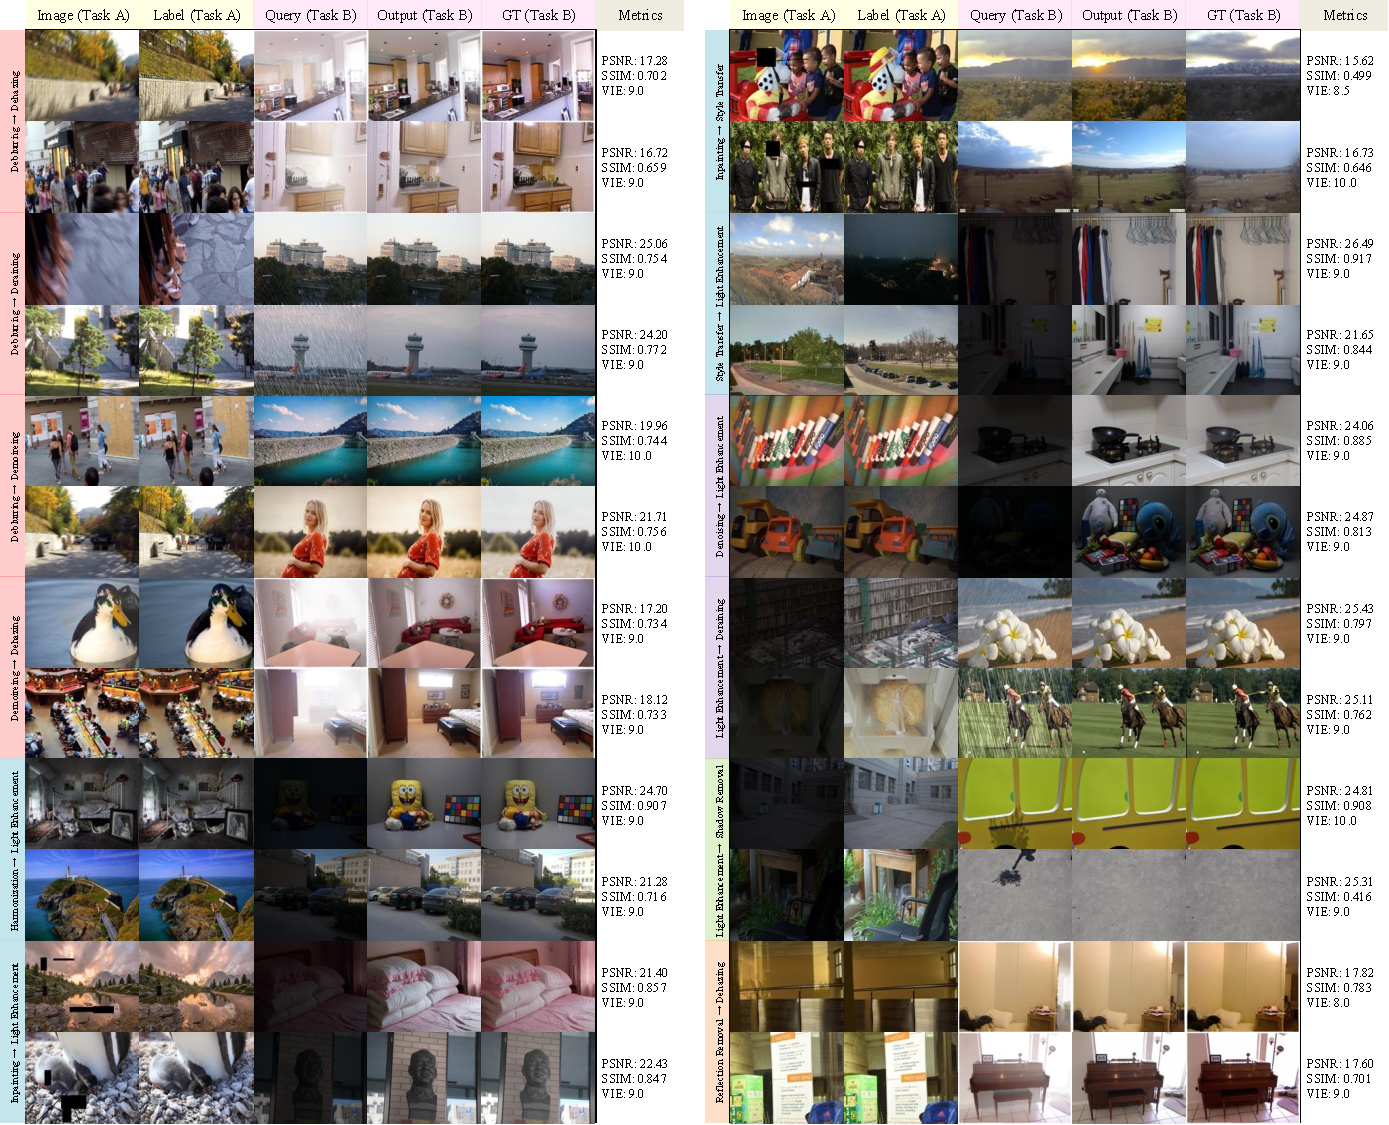
\includegraphics[width=\textwidth]{fig/figure4.pdf}
    \caption{Representative Examples of Cross-Task In-Context Learning from Gemini in Twelve Pairs}
    \label{fig:fig4}
\vspace{-8pt}
\end{figure*}

\subsection{Cross-Task Diversity and Adaptability}
The proposed VICL demonstrates consistent gains across diverse low-level vision tasks such as dehazing, deraining, demoireing. Beyond, the same prompting mechanism seamlessly extends to generation-oriented tasks such as low-light enhancement, effectively maintaining spatial layout and identity fidelity. Unlike prior approaches that are often confined to semantically similar domains, our method adapts seamlessly across both intra-category tasks (e.g., harmonization vs. light enhancement, demoireing vs. dehazing) and inter-category tasks (e.g., reflection removal vs. dehazing). These findings highlight the scalability and flexibility of our approach, showing that T2T-VICL can naturally bridge both perceptually related and unrelated tasks under a single model.

\subsection{Generalization to Distant Tasks} Beyond absolute numbers, an important property is cross-task consistency. This consistency underlines the advantage of framing all tasks under a unified in-context prompting mechanism. Moreover, T2T-VICL generalizes to semantically distant task pairs such as denoising versus light enhancement, where task-specialized models tend to degrade without task-specific retraining. This highlights robustness as a key byproduct of the unified in-context paradigm.

% \begin{table*}[ht]
% \centering
% \captionsetup{width=0.78\textwidth, skip=4pt, type=table}
% \caption{Average of evaluation metrics in the second-tier group. Generated by Gemini with Qwen prompts, compared to the fixed-prompt baseline.}
% \vspace{-1pt}

% \small
% % \scriptsize
% % \setlength{\tabcolsep}{4pt}
% % \renewcommand{\arraystretch}{1.0}

% \begin{tabularx}{0.785\textwidth}{lcccccc}
% \toprule
% \multirow{2}{*}{\textbf{Task}} & \multicolumn{2}{c}{\textbf{PSNR}$\uparrow$} & \multicolumn{2}{c}{\textbf{SSIM}$\uparrow$} & \multicolumn{2}{c}{\textbf{VIEScore}$\uparrow$} \\
%  & \textcolor{gray}{\textbf{Fixed}} & \textcolor{gray}{\textbf{Ours}}
%  & \textcolor{gray}{\textbf{Fixed}} & \textcolor{gray}{\textbf{Ours}}
%  & \textcolor{gray}{\textbf{Fixed}} & \textcolor{gray}{\textbf{Ours}} \\
% \midrule

% \rowcolor{lightred!30}
% Dehazing $\rightarrow$ Deraining             & \cellcolor{lightred!60}19.09 & 19.01 & \cellcolor{lightred!60}0.518 & 0.505 & 6.39 & \cellcolor{lightred!60}7.13 \\
% \rowcolor{lightred!30}
% Deraining $\rightarrow$ Demoireing             & \cellcolor{lightred!60}15.29 & 15.00 & \cellcolor{lightred!60}0.583 & 0.580 & 5.83 & \cellcolor{lightred!60}7.24 \\
% \rowcolor{lightblue!30}
% Colorization $\rightarrow$ Style Transfer    & \cellcolor{lightblue!60}13.35 & 13.03 & \cellcolor{lightblue!60}0.465 & 0.434 & 5.10 & \cellcolor{lightblue!60}7.37 \\
% \rowcolor{lightblue!30}
% Harmonization $\rightarrow$ Style Transfer   & \cellcolor{lightblue!60}13.32 & 13.14 & \cellcolor{lightblue!60}0.465 & 0.458 & 4.79 & \cellcolor{lightblue!60}5.66 \\
% \rowcolor{lightblue!30}
% Inpainting $\rightarrow$ Colorization        & \cellcolor{lightblue!60}21.31 & 20.75 & \cellcolor{lightblue!60}0.843 & 0.742 & 5.23 & \cellcolor{lightblue!60}7.39 \\
% \rowcolor{lightblue!30}
% Light Enhancement $\rightarrow$ Colorization & \cellcolor{lightblue!60}22.72 & 21.04 & \cellcolor{lightblue!60}0.860 & 0.753 & 5.05 & \cellcolor{lightblue!60}6.86 \\
% \rowcolor{lightpurple!30}
% Deraining $\rightarrow$ Style Transfer       & \cellcolor{lightpurple!60}13.31 & 13.10 & 0.430 & \cellcolor{lightpurple!60}0.447 & 4.67 & \cellcolor{lightpurple!60}5.66 \\
% \rowcolor{lightorange!30}
% Shadow Removal $\rightarrow$ Deraining       & \cellcolor{lightorange!50}19.49 & 18.98 & \cellcolor{lightorange!50}0.555 & 0.538 & 7.54 & \cellcolor{lightorange!50}8.20 \\
% \rowcolor{lightyellow!30}
% Shadow Removal $\rightarrow$ Reflection Removal & \cellcolor{lightyellow!50}21.79 & 21.44 & \cellcolor{lightyellow!50}0.761 & 0.739 & 6.24 & \cellcolor{lightyellow!50}6.34 \\
% \bottomrule
% \end{tabularx}
% \end{table*}



\begin{table*}[ht]
\centering
\scriptsize
\setlength{\tabcolsep}{0.5pt}
\renewcommand{\arraystretch}{0.96}
\captionsetup{width=0.98\textwidth, skip=4pt, type=table}
\caption{Average of evaluation metrics in the second-tier group. Generated by Gemini and Seedream with Qwen prompts, compared to the fixed-prompt baseline.}
% These task pairs consistently improve VIEScore for both Gemini and Seedream, while PSNR or SSIM may decrease.
\vspace{-1pt}
\label{tab:4}

\begin{adjustbox}{width=\textwidth}
\begin{tabular}{H *{5}{>{\centering\arraybackslash}m{0.8cm}} >{\centering\arraybackslash}m{1cm} *{5}{>{\centering\arraybackslash}m{0.8cm}} >{\centering\arraybackslash}m{1cm}}
\toprule
\multirow{3}{*}{\textbf{Task}}
& \multicolumn{6}{c}{\textbf{Gemini 2.5 Flash}}
& \multicolumn{6}{c}{\textbf{Seedream 4.0}} \\
& \multicolumn{2}{c}{\textbf{PSNR}$\uparrow$}
& \multicolumn{2}{c}{\textbf{SSIM}$\uparrow$}
& \multicolumn{2}{c}{\textbf{VIEScore}$\uparrow$}
& \multicolumn{2}{c}{\textbf{PSNR}$\uparrow$}
& \multicolumn{2}{c}{\textbf{SSIM}$\uparrow$}
& \multicolumn{2}{c}{\textbf{VIEScore}$\uparrow$} \\
& \textcolor{gray}{\textbf{Fixed}} & \textcolor{gray}{\textbf{Ours}}
& \textcolor{gray}{\textbf{Fixed}} & \textcolor{gray}{\textbf{Ours}}
& \textcolor{gray}{\textbf{Fixed}} & \textcolor{gray}{\textbf{Ours}}
& \textcolor{gray}{\textbf{Fixed}} & \textcolor{gray}{\textbf{Ours}}
& \textcolor{gray}{\textbf{Fixed}} & \textcolor{gray}{\textbf{Ours}}
& \textcolor{gray}{\textbf{Fixed}} & \textcolor{gray}{\textbf{Ours}} \\
\midrule

\rowcolor{lightred!30}
\makecell[l]{Dehazing $\rightarrow$ Deraining}
& \cellcolor{lightred!60}19.09 & 19.01
& \cellcolor{lightred!60}0.518 & 0.505
& 6.39 & \cellcolor{lightred!60}\tabgainsubscript{7.13}{+0.74}
& 14.47 & \cellcolor{lightred!60}14.49
& 0.385 & \cellcolor{lightred!60}0.386
& 6.41 & \cellcolor{lightred!60}\tabgainsubscript{6.76}{+0.35} \\
\grayhline

\rowcolor{lightred!30}
\makecell[l]{Deraining $\rightarrow$ Demoireing}
& \cellcolor{lightred!60}15.29 & 15.00
& \cellcolor{lightred!60}0.583 & 0.580
& 5.83 & \cellcolor{lightred!60}\tabgainsubscript{7.24}{+1.41}
& \cellcolor{lightred!60}11.84 & 10.95
& \cellcolor{lightred!60}0.451 & 0.418
& 7.38 & \cellcolor{lightred!60}\tabgainsubscript{7.40}{+0.02} \\
\grayhline

\rowcolor{lightblue!30}
\makecell[l]{Colorization $\rightarrow$ Style Transfer}
& \cellcolor{lightblue!60}13.35 & 13.03
& \cellcolor{lightblue!60}0.465 & 0.434
& 5.10 & \cellcolor{lightblue!60}\tabgainsubscript{7.37}{+2.27}
& \cellcolor{lightblue!60}9.91 & 9.54
& \cellcolor{lightblue!60}0.333 & 0.314
& 7.99 & \cellcolor{lightblue!60}\tabgainsubscript{8.09}{+0.10} \\
\grayhline

\rowcolor{lightblue!30}
\makecell[l]{Harmonization $\rightarrow$ Style Transfer}
& \cellcolor{lightblue!60}13.32 & 13.14
& \cellcolor{lightblue!60}0.465 & 0.458
& 4.79 & \cellcolor{lightblue!60}\tabgainsubscript{5.66}{+0.87}
& \cellcolor{lightblue!60}10.20 & 9.63
& \cellcolor{lightblue!60}0.354 & 0.331
& 7.32 & \cellcolor{lightblue!60}\tabgainsubscript{7.62}{+0.30} \\
\grayhline

\rowcolor{lightblue!30}
\makecell[l]{Inpainting $\rightarrow$ Colorization}
& \cellcolor{lightblue!60}21.31 & 20.75
& \cellcolor{lightblue!60}0.843 & 0.742
& 5.23 & \cellcolor{lightblue!60}\tabgainsubscript{7.39}{+2.16}
& \cellcolor{lightblue!60}13.53 & 12.08
& \cellcolor{lightblue!60}0.447 & 0.397
& 5.86 & \cellcolor{lightblue!60}\tabgainsubscript{6.96}{+1.10} \\
\grayhline

\rowcolor{lightblue!30}
\makecell[l]{Light Enhancement $\rightarrow$ Colorization}
& \cellcolor{lightblue!60}22.72 & 21.04
& \cellcolor{lightblue!60}0.860 & 0.753
& 5.05 & \cellcolor{lightblue!60}\tabgainsubscript{6.86}{+1.81}
& 11.01 & \cellcolor{lightblue!60}12.09
& \cellcolor{lightblue!60}0.436 & 0.422
& 4.59 & \cellcolor{lightblue!60}\tabgainsubscript{7.28}{+2.69} \\
\grayhline

\rowcolor{lightyellow!30}
\makecell[l]{Shadow Removal $\rightarrow$ Reflection Removal}
& \cellcolor{lightyellow!50}21.79 & 21.44
& \cellcolor{lightyellow!50}0.761 & 0.739
& 6.24 & \cellcolor{lightyellow!50}\tabgainsubscript{6.34}{+0.10}
& \cellcolor{lightyellow!50}14.96 & 13.10
& \cellcolor{lightyellow!50}0.532 & 0.459
& 7.13 & \cellcolor{lightyellow!50}\tabgainsubscript{7.17}{+0.04} \\
\grayhline

\rowcolor{lightpurple!30}
\makecell[l]{Deraining $\rightarrow$ Style Transfer}
& \cellcolor{lightpurple!60}13.31 & 13.10
& 0.430 & \cellcolor{lightpurple!60}0.447
& 4.67 & \cellcolor{lightpurple!60}\tabgainsubscript{5.66}{+0.99}
& \cellcolor{lightpurple!60}11.02 & 9.76
& \cellcolor{lightpurple!60}0.375 & 0.318
& 6.66 & \cellcolor{lightpurple!60}\tabgainsubscript{7.33}{+0.67} \\
\grayhline

\rowcolor{lightorange!30}
\makecell[l]{Shadow Removal $\rightarrow$ Deraining}
& \cellcolor{lightorange!50}19.49 & 18.98
& \cellcolor{lightorange!50}0.555 & 0.538
& 7.54 & \cellcolor{lightorange!50}\tabgainsubscript{8.20}{+0.66}
& \cellcolor{lightorange!50}17.37 & 15.25
& \cellcolor{lightorange!50}0.487 & 0.431
& 7.51 & \cellcolor{lightorange!50}\tabgainsubscript{7.68}{+0.17} \\
\bottomrule
\end{tabular}
\end{adjustbox}
\vspace{-6pt}
\end{table*}


\subsection{Cross-Task Results in Second-Tier Group}
Across another nine cross-task pairs in Table~\ref{tab:4}, our method consistently improves VIEScore over the fixed-prompt baseline on both Gemini and Seedream. The other two IQA metrics have slight declines in several cases. Interestingly, for these compositions, improvements are primarily reflected in the VIEScore rather than in the traditional fidelity metrics. Since VIE measures structural and relational coherence of visual information, it is more sensitive to semantic preservation than to strict intensity alignment. See detailed discussion in Appendix Sec.~\ref{sec:viescore}.

% \vspace{1pt}
% \noindent
% \begin{minipage}{\columnwidth}
% \centering
% \captionsetup{font=scriptsize, width=\columnwidth, skip=1pt}
% \captionof{table}{Avg of metrics for ablation study on effects of prompt enhancement and ICL.}
% % (1) One input image + training data copied long fixed prompt;
% % (2) Image 1-3 all from same task, clear fixed prompt (same task);
% % (3) Image 1-3 all from same task, long prompt (image descriptions + visual changes).
% \label{tab:r2}
% \scriptsize
% \setlength{\tabcolsep}{1.48pt}
% \renewcommand{\arraystretch}{0.927}
% \begin{tabularx}{\columnwidth}{S*{9}{C}}
% \toprule
% \multirow{2}{*}{\textbf{Task}} 
% & \multicolumn{3}{c}{\textbf{Prompt-only}} 
% & \multicolumn{3}{c}{\textbf{Same-task ICL+Fix}} 
% & \multicolumn{3}{c}{\textbf{Same-task ICL+Enh}} \\
% & PSNR & SSIM & VIE
% & PSNR & SSIM & VIE
% & PSNR & SSIM & VIE \\
% \midrule

% \rowcolor{lightred!30}
% Deblurring
% & 20.14 & 0.597 & 4.66
% & 17.51 & 0.529 & \cellcolor{lightred!60}4.69
% & \cellcolor{lightred!60}19.29 & \cellcolor{lightred!60}0.578 & 4.30 \\

% \rowcolor{lightred!30}
% Dehazing
% & 13.08 & 0.541 & 8.05
% & 12.47 & 0.510 & 6.78
% & \cellcolor{lightred!60}12.68 & \cellcolor{lightred!60}0.511 & \cellcolor{lightred!60}6.92 \\

% \rowcolor{lightred!30}
% Demoireing
% & 15.88 & 0.588 & 8.87
% & 14.98 & 0.574 & 7.41
% & \cellcolor{lightred!60}15.89 & \cellcolor{lightred!60}0.596 & \cellcolor{lightred!60}7.57 \\

% \rowcolor{lightred!30}
% Deraining
% & 20.40 & 0.591 & 8.62
% & 19.61 & 0.563 & 7.31
% & \cellcolor{lightred!60}19.86 & \cellcolor{lightred!60}0.575 & \cellcolor{lightred!60}8.00 \\

% \rowcolor{lightblue!30}
% Colorization
% & 20.61 & 0.722 & 8.69
% & \cellcolor{lightblue!60}21.18 & \cellcolor{lightblue!60}0.788 & 6.51
% & 20.68 & 0.755 & \cellcolor{lightblue!60}7.29 \\

% \rowcolor{lightblue!30}
% Harmonization
% & 19.71 & 0.592 & 9.77
% & 19.88 & 0.648 & \cellcolor{lightblue!60}6.65
% & \cellcolor{lightblue!60}20.18 & \cellcolor{lightblue!60}0.662 & 6.61 \\

% \rowcolor{lightblue!30}
% Inpainting
% & 18.81 & 0.516 & 9.12
% & 18.18 & 0.544 & 8.31
% & \cellcolor{lightblue!60}18.81 & \cellcolor{lightblue!60}0.547 & \cellcolor{lightblue!60}8.65 \\

% \rowcolor{lightblue!30}
% Light Enh.
% & 14.37 & 0.576 & 8.98
% & 12.27 & 0.482 & 8.26
% & \cellcolor{lightblue!60}14.00 & \cellcolor{lightblue!60}0.574 & \cellcolor{lightblue!60}8.92 \\

% \rowcolor{lightblue!30}
% Style Trans.
% & 13.24 & 0.444 & 8.58
% & 12.96 & \cellcolor{lightblue!60}0.452 & \cellcolor{lightblue!60}6.69
% & \cellcolor{lightblue!60}13.08 & 0.446 & 6.42 \\

% \rowcolor{lightyellow!30}
% Refl. Rmv.
% & 22.19 & 0.753 & 7.78
% & 20.13 & 0.718 & 5.84
% & \cellcolor{lightyellow!60}22.25 & \cellcolor{lightyellow!60}0.766 & \cellcolor{lightyellow!60}5.90 \\

% \rowcolor{lightyellow!30}
% Shadow Rmv.
% & 19.19 & 0.338 & 8.87
% & \cellcolor{lightyellow!60}18.72 & \cellcolor{lightyellow!60}0.334 & 7.47
% & 18.58 & 0.333 & \cellcolor{lightyellow!60}8.31 \\

% \bottomrule
% \end{tabularx}
% \end{minipage}
% \vspace{-4pt}


\vspace{6pt}
\noindent
\begin{minipage}{\columnwidth}
\centering
\captionsetup{width=0.99\columnwidth, skip=4pt, type=table}
\captionof{table}{Average of metrics for ablation study on effects of prompt enhancement and ICL, generated by Gemini.}
% (1) One input image + training data copied long fixed prompt;
% (2) Image 1-3 all from same task, clear fixed prompt (same task);
% (3) Image 1-3 all from same task, long prompt (image descriptions + visual changes).
\label{tab:6}
\scriptsize
\setlength{\tabcolsep}{2pt}
\renewcommand{\arraystretch}{0.95}
\begin{tabularx}{\columnwidth}{l*{6}{C}}
\toprule
\multirow{2}{*}{\textbf{Task}} 
% & \multicolumn{3}{c}{\textbf{Prompt-only}} 
& \multicolumn{3}{c}{\textbf{Same-task ICL + Fixed}} 
& \multicolumn{3}{c}{\textbf{Same-task ICL + Enh.}} \\
% & PSNR & SSIM & VIE
& PSNR & SSIM & VIE
& PSNR & SSIM & VIE \\
\midrule

\rowcolor{lightred!30}
Deblurring
% & 20.14 & 0.597 & 4.66
& 17.51 & 0.529 & \cellcolor{lightred!60}4.69
& \cellcolor{lightred!60}19.29 & \cellcolor{lightred!60}0.578 & 4.30 \\

\rowcolor{lightred!30}
Dehazing
% & 13.08 & 0.541 & 8.05
& 12.47 & 0.510 & 6.78
& \cellcolor{lightred!60}12.68 & \cellcolor{lightred!60}0.511 & \cellcolor{lightred!60}6.92 \\

\rowcolor{lightred!30}
Demoireing
% & 15.88 & 0.588 & 8.87
& 14.98 & 0.574 & 7.41
& \cellcolor{lightred!60}15.89 & \cellcolor{lightred!60}0.596 & \cellcolor{lightred!60}7.57 \\

\rowcolor{lightred!30}
Deraining
% & 20.40 & 0.591 & 8.62
& 19.61 & 0.563 & 7.31
& \cellcolor{lightred!60}19.86 & \cellcolor{lightred!60}0.575 & \cellcolor{lightred!60}8.00 \\

\rowcolor{lightblue!30}
Colorization
% & 20.61 & 0.722 & 8.69
& \cellcolor{lightblue!60}21.18 & \cellcolor{lightblue!60}0.788 & 6.51
& 20.68 & 0.755 & \cellcolor{lightblue!60}7.29 \\

\rowcolor{lightblue!30}
Harmonization
% & 19.71 & 0.592 & 9.77
& 19.88 & 0.648 & \cellcolor{lightblue!60}6.65
& \cellcolor{lightblue!60}20.18 & \cellcolor{lightblue!60}0.662 & 6.61 \\

\rowcolor{lightblue!30}
Inpainting
% & 18.81 & 0.516 & 9.12
& 18.18 & 0.544 & 8.31
& \cellcolor{lightblue!60}18.81 & \cellcolor{lightblue!60}0.547 & \cellcolor{lightblue!60}8.65 \\

\rowcolor{lightblue!30}
Light Enhancement
% & 14.37 & 0.576 & 8.98
& 12.27 & 0.482 & 8.26
& \cellcolor{lightblue!60}14.00 & \cellcolor{lightblue!60}0.574 & \cellcolor{lightblue!60}8.92 \\

\rowcolor{lightblue!30}
Style Transfer
% & 13.24 & 0.444 & 8.58
& 12.96 & \cellcolor{lightblue!60}0.452 & \cellcolor{lightblue!60}6.69
& \cellcolor{lightblue!60}13.08 & 0.446 & 6.42 \\

\rowcolor{lightyellow!30}
Reflection Removal
% & 22.19 & 0.753 & 7.78
& 20.13 & 0.718 & 5.84
& \cellcolor{lightyellow!60}22.25 & \cellcolor{lightyellow!60}0.766 & \cellcolor{lightyellow!60}5.90 \\

\rowcolor{lightyellow!30}
Shadow Removal
% & 19.19 & 0.338 & 8.87
& \cellcolor{lightyellow!60}18.72 & \cellcolor{lightyellow!60}0.334 & 7.47
& 18.58 & 0.333 & \cellcolor{lightyellow!60}8.31 \\

\bottomrule
\end{tabularx}
% \vspace{3pt}
\end{minipage}


\subsection{Ablation Study}

We further investigate the scalability of our method under the traditional same-task VICL setting. Specifically, we conduct ablation studies on Gemini to validate the performance gains of T2T-VICL by: (1) applying VICL to the same task with a fixed prompt, and (2) applying VICL to the same task with an implicitly enriched prompt derived from same task samples using a similar pipeline as T2T-VICL. 
Details of the two prompt configurations are provided in Sec.~\ref{sec:prompt} in Appendix.
Table~\ref{tab:6} reports the results of same-task VICL with fixed and enhanced prompts.
Experimental results demonstrate improvements in PSNR, SSIM, and VIEScore across multiple task pairs.


\subsection{Discussion}
Overall, our framework demonstrates strong one-shot generalization and robust visual consistency across a wide range of low-level vision tasks. By leveraging implicit prompt representations, the model effectively adapts to unseen task combinations without task-specific fine-tuning, achieving top-tier VIEScores in many cases. However, due to the inherent complexity of cross-task compositions, a few cases with limited reference samples occasionally produce content that does not exist in the original images, slightly lowering the fidelity-based indicators. Despite these imperfections, the overall visual consistency remains close to that of the top group. Future work will focus on adaptive balancing between semantic-level and pixel-level objectives to further improve realism and generalization across diverse unseen conditions.

\section{Conclusion}
\label{sec:concl}

In conclusion, we propose the first cross-task visual in-context learning pipeline, i.e T2T-VICL, that enables collaboration among multiple VLMs, together with an automatic reasoning mechanism. Our framework systematically explores the largely uncharted boundaries of cross-task transfer in VICL. This collaborative paradigm fills a gap in understanding how heterogeneous VLMs can jointly reason and adapt across tasks, and we anticipate that our findings will encourage further investigation into the mechanisms that underpin cross-task transfer and the broader generalization capacity of multimodal models.


\section*{Limitations}
Since our scope is primarily on low-level vision tasks, we select 12 representative low-level tasks, covering most commonly studied low-level tasks in the literature and exceeding the task coverage of many VICL or prompt-enhanced works in this field (e.g., MAE-VQGAN 3,  Painter 3, ProRes 4,  PromptIR 3, InstructIR 8). It is notable the number of cross-task experiments grows quadratically with the number of tasks, compared to same-task VICL, we will consider more niche tasks in the future. In some representative higher-level tasks, such as geometric problem-solving and spatial reasoning, VLMs may exhibit weak baseline performance, thus the practical applicability of our approach in these scenarios still require further investigation.
Meantime, task transfer capability in VLMs is not unlimited and might depend on underlying similarity of low-level tasks. Our results indicate implicit task transfer is feasible but also constrained, which is partially consistent with previous studies such as Taskonomy~\cite{zamir2018taskonomy}.

% \section*{Acknowledgments}

\clearpage
\bibliography{ref}

\appendix
\clearpage

\section*{Appendix}
\label{sec:appendix}
% \setcounter{section}{0}   

\section{Dataset Details}
\label{sec:data}

We build our T2T-VICL benchmark by assembling representative paired datasets for a wide set of low-level image processing tasks. For each task we use well-known, publicly available datasets without altering their ground-truth semantics; where appropriate we apply lightweight, clearly documented preprocessing so that training and evaluation are consistent across tasks. The particular dataset selection and provenance mirror those reported in the main paper. The following subsections detail the origin of each dataset, the typical size\slash resolution, and the data split employed in our experiments.

\subsection{Per-Dataset Descriptions}
\noindent \textbf{GOPRO (deblurring).} We use this large motion deblurring dataset introduced for dynamic scene deblurring; it contains 3,214 blurry and sharp pairs captured from high-speed video and typically provided at 1280 $\times$ 720 resolution. This dataset provides realistic, non-uniform motion blur that matches the ``motion-blur restoration'' scenario in our cross-task experiments.

\noindent \textbf{D-HAZY (dehazing).} D-HAZY is a synthetic dehazing dataset produced by applying Koschmieder atmospheric scattering model to images with depth (e.g., images from Middlebury and NYU Depth datasets); it contains on the order of 1,400+ hazy\slash haze-free image pairs and is widely used to benchmark single-image dehazing approaches. We use the official image pairs and follow the commonly used splits reported by the dataset authors.

\noindent \textbf{UHDM (demoireing).} We use the UHDM ultra-high-definition demoireing dataset, which is composed of 5,000 real 4K image pairs collected for moire removal and scale-robust evaluation. UHDM is appropriate for demoireing examples in our benchmark because it contains diverse real-world moire patterns at 4K scale. In practice we downsample/crop to the model's working size for training while retaining high-resolution examples for qualitative figures.

\noindent \textbf{SIDD (denoising).} The Smartphone Image Denoising Dataset (SIDD) provides real noisy smartphone photographs and matching ground truth; the dataset contains roughly $\sim$30,000 noisy images which are generated from multiple scenes and devices and is the standard benchmark for real-world image denoising. We use the released training and benchmark splits for denoising experiments.

\noindent \textbf{RainCityscapes (deraining).} RainCityscapes is built on Cityscapes imagery and provides synthetically generated rainy variants with depth maps; the commonly cited partition includes thousands of rainy/clean images pairs. We use RainCityscapes for deraining A $\rightarrow$ B pairs since it contains realistic outdoor scenes with varying rain density.

\noindent \textbf{iHarmony4 (harmonization).} iHarmony4 is a large image harmonization benchmark composed of four sub-datasets (HCOCO, HAdobe5k, HFlickr, and Hday2night) that together provide tens of thousands of composed images and corresponding real images. We pick the Hday2night set for harmonization experiments.

\noindent \textbf{DIV2K (inpainting, colorization).} DIV2K contains 1,000 high-quality 2K images with a large diversity of contents. For inpainting and colorization experiments we use DIV2K images with controlled masking or decolorization pipelines to create paired inputs and targets as the original images come naturally as the ground truth images.

\noindent \textbf{LoL (light enhancement).} The original LoL (low-light) dataset provides paired low/normal light images; the common LoL-v1 split contains 500 image pairs. We adopt the same pairs and the standard split.

\noindent \textbf{SIR$^2$ (reflection removal).} The SIR$^2$ benchmark provides controlled and wild scenes with ground-truth background/reflection separation. We use the SIR$^2$ ground-truth pairs for reflection removal examples.

\noindent \textbf{ISTD (shadow removal).} The ISTD (Image Shadow Triplets) dataset dataset for shadow understanding contains 1,870 pairs of shadow and shadow-free images. We use the ISTD triplets for all shadow removal A $\rightarrow$ B evaluations.

\noindent \textbf{Night2Day (style transfer).} For style transfer, we use publicly available unpaired dataset commonly referred to as Night2Day, which includes images of outdoor scenes with various appearances such as snow, autumn, dusk, and fog. Depending on the data, we paired images related to the same scene with different appearances ourselves to construct image pairs required for our experiments.

\noindent \textbf{Note on splits \& preprocessing.} For each dataset above we kept the data processing code. Especially for synthetic variants (e.g., DIV2K $\rightarrow$ inpainting/colorization data), we document the exact generation protocol in the dataset code which will be published after this submission.

\subsection{Pair Construction for Cross-Task}
For every source dataset (task A dataset) we sample N examples and pair them with N examples drawn from target dataset (task B dataset) to form cross-task demonstration pairs. To maximize the diversity of implicit descriptions used to teach the sVLM, we generate candidate teacher texts for many different task A/B examples and then apply embedding-based clustering and deduplication to retain high-variance, information-rich implicit prompts.


\section{Prompt Design}
\label{sec:prompt}

Two different conditioning strategies are compared in our experiments: (1) a fixed template prompt that merely describes the I/O demonstration structure (instruction: ``what is shown and what to do''), and (2) implicit prompts generated at inference time by the fine-tuned Qwen student model that describe visual differences and transformation goals between the provided Task A input/output pair and the Task B query input, but crucially without naming tasks explicitly. The implicit prompt therefore acts as a content-dependent, transformation-specific instruction that guides the downstream VLM to adapt the example transformation to the new input. This design is central to T2T-VICL's ability to perform cross-task visual in-context learning.

\subsection{Fixed Prompt}
We used the following fixed prompt as baseline (this is the exact wording used in our fixed-prompt experiments):

\begin{tcolorbox}[colback=gray!20, colframe=gray!20, boxrule=0pt, left=3pt, right=3pt, top=3pt, bottom=3pt]
\emph{This is a visual in-context learning task. The first two images are an input and output of Task A. The third image is the input for Task B. The goal is to perform Task B on the third image and generate an output image, learning from Task A.}
\end{tcolorbox}

\noindent This fixed prompt provides clear structural cues but does not communicate task-specific differences, e.g., whether the change is about removing linear occlusions vs. suppressing uniform noise. Therefore, it acts as a conservative baseline for comparing the benefit of more descriptive (implicit) instructions.

\noindent Similarly, the fixed prompt applied in the same-task VICL for the ablation study is as follows:

\begin{tcolorbox}[colback=gray!20, colframe=gray!20, boxrule=0pt, left=3pt, right=3pt, top=3pt, bottom=3pt]
\emph{This is a visual in-context learning task. The first two images are an input and output of an image processing task. The third image is the input for the SAME task. The goal is to perform this task on the third image and generate an output image, learning from the pair before.}
\end{tcolorbox}

\subsection{Implicit Prompt (Qwen)}
\textbf{How it is created.} For each sampled A $\rightarrow$ B tuple ($I_A^{in}$, $I_A^{l}$, $I_B^{in}, I_B^l$), a large teacher VLM is prompted with four images and an open-ended instruction (``Compare the effects observed in these images and produce a descriptive instruction that would allow another model to transform $I_B^{in}$ into $I_B^{out}$''), which elicits a rich, descriptive text. These candidate texts are post-processed (clustering\slash de-duplication\slash filtering) to keep high-variance, informative implicit prompts which are then used as training targets for our small sVLM (Qwen3-VL-4B) to learn to generate such implicit prompts given similar image triples.

\noindent \textbf{What the implicit prompt contains.} Typical implicit prompts contain three types of information: (1) target goals (what visual attributes should be achieved in the output), (2) input degradation description (what to remove/mitigate), and (3) how to change visual statistics (e.g., preserve texture, restore local contrast, avoid color casts). Importantly the language avoids direct task names (no explicit ``derain/denoise/deblur'' tokens), which forces the model to rely on visual-descriptive cues and allows transferring the transformation style across tasks.

\noindent \textbf{Why it helps.} Because the implicit prompt encodes the target visual change in fine-grained, task-agnostic language, it provides the downstream generator with actionable, content-sensitive guidance. This guidance improves adaptation when the transformation required by Task B differs in surface form from Task A, yet still shares similar latent transformation principles.

\noindent \textbf{Example.}
Below we give one long, representative teacher output used as an illustrative example in the supplementary. This example is intentionally verbose to demonstrate the kinds of distinctions the implicit prompt encodes; a single long instruction like this is used as a training target for sVLM.

\begin{tcolorbox}[colback=gray!20, colframe=gray!20, boxrule=0pt, left=3pt, right=3pt, top=3pt, bottom=3pt]

\emph{This is a visual in-context learning task. The first two images are an input and output of Task A. The third image is the input for Task B. The goal is to perform Task B on the third image and generate an output image, learning from Task A.}
\vspace{1pt}

\emph{\textbf{Analysis of Tasks A and B}}

% \emph{\textbf{Input Image Descriptions}}
\emph{\textbf{Input Descriptions}}

\begin{itemize}

\item \emph{\textbf{Task A:} The input image shows a dimly lit room with stacked boxes containing various items, including a basketball. The lighting is low, making details difficult to discern.}

\item \emph{\textbf{Task B:} The input image is a black-and-white photograph of a person wearing sunglasses and a headscarf, holding a phone to their ear. The image lacks color and has a monochromatic tone.}

\end{itemize}

\emph{\textbf{Visual Changes}}

\begin{itemize}

\item \emph{\textbf{Task A:} The output image is brighter, with improved lighting that enhances visibility and detail of the objects within the room.}

\item \emph{\textbf{Task B:} The output image is in color, transforming the black-and-white photo into a full-color representation, adding vibrancy and depth.}

\end{itemize}

% \emph{\textbf{Differences of Tasks}}
\emph{\textbf{Task Differences}}

\begin{itemize}

\item \emph{\textbf{Task A:} Task A focuses on enhancing brightness and visibility, likely through illumination or contrast adjustments.}

\item \emph{\textbf{Task B:} Task B emphasizes color restoration, converting a grayscale image into a colorful one, which alters the overall aesthetic and provides more visual information.}

\end{itemize}

\end{tcolorbox}

\noindent Similarly, one example of implicitly enhanced prompt in the ablation study section is (Note: same-task VICL does not have the Task Differences item):

\begin{tcolorbox}[colback=gray!20, colframe=gray!20, boxrule=0pt, left=3pt, right=3pt, top=3pt, bottom=3pt]

\emph{This is a visual in-context learning task. The first two images are an input and output of an image processing task. The third image is the input for the same task. The goal is to perform this task on the third image and generate an output image, learning from the pair before.}

\end{tcolorbox}

\begin{tcolorbox}[colback=gray!20, colframe=gray!20, boxrule=0pt, left=3pt, right=3pt, top=3pt, bottom=3pt]

\emph{\textbf{Image Descriptions}}

\emph{Picture 1 shows a monochrome shot of a racer on a motorcycle, while Picture 2 presents the same scene with vibrant, saturated colors restored.}

\emph{\textbf{Visual Changes}}

\emph{The task transforms the grayscale representation into a vivid, full-color depiction, enhancing the visual richness and detail of the subject.}

\emph{The third image, a grayscale kite on grass, would similarly gain vivid color saturation to match the enhanced palette of the first two images.}

\end{tcolorbox}


\section{Inference Details}
\label{sec:infer}

Figure~\ref{fig:fig3} gives a concrete inference-stage example to clarify how the fixed prompt and the implicit prompt are used. Both settings receive the same visual inputs: an input-output demonstration pair from task A and a query input from task B.
T2T-VICL first asks the trained sVLM to produce an implicit prompt from the same images, and the generated prompt is then concatenated with the fixed structural instruction and passed, together with the images, to the frozen VLM.
The figure visualizes this complete route from visual prompt construction to final output, showing why the implicit prompt serves as an interpretable bridge between a task-A demonstration and a task-B query.

\begin{figure*}[t]
    \centering
    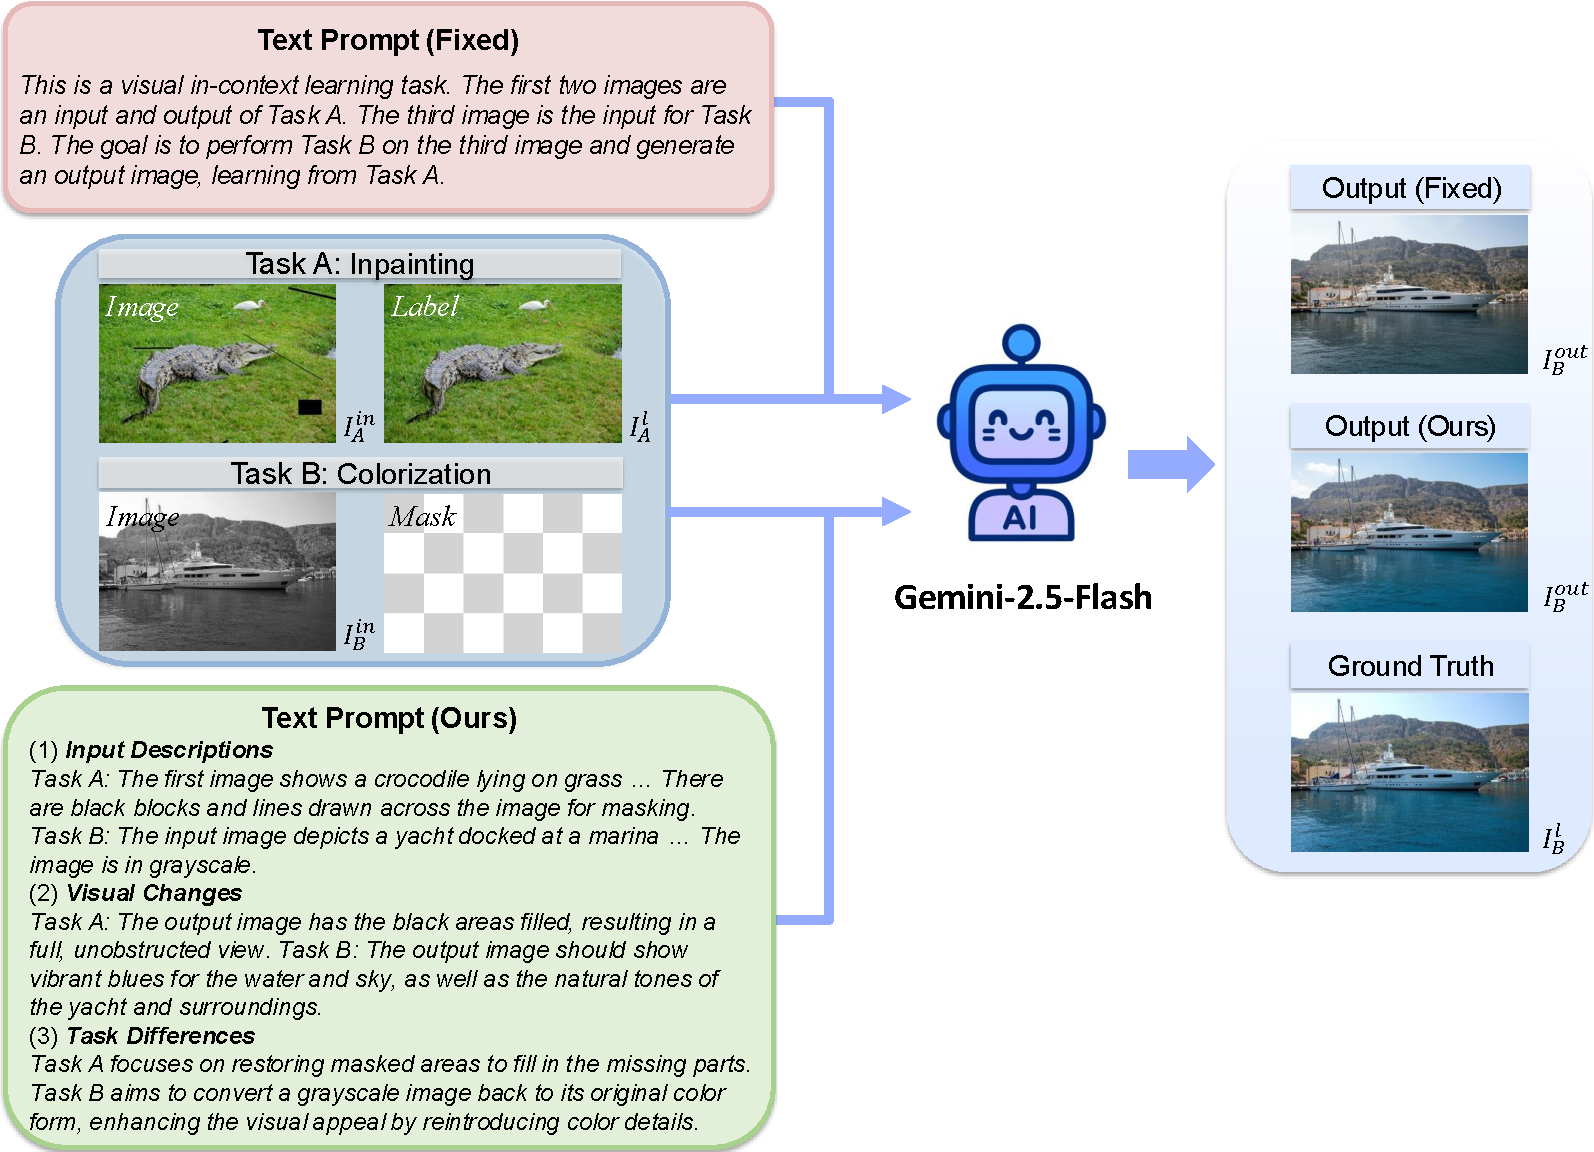
\includegraphics[width=0.9\textwidth]{fig/figure3.pdf}
    \caption{Detailed Example of Cross-Task Visual In-Context Learning in Inference Stage}
    \label{fig:fig3}
\vspace{-8pt}
\end{figure*}


\section{Additional Results and Analysis}

% \subsection{Cross-Task Qualitative Results}
% \label{sec:example}

% \begin{figure*}[ht]
%     \centering
%     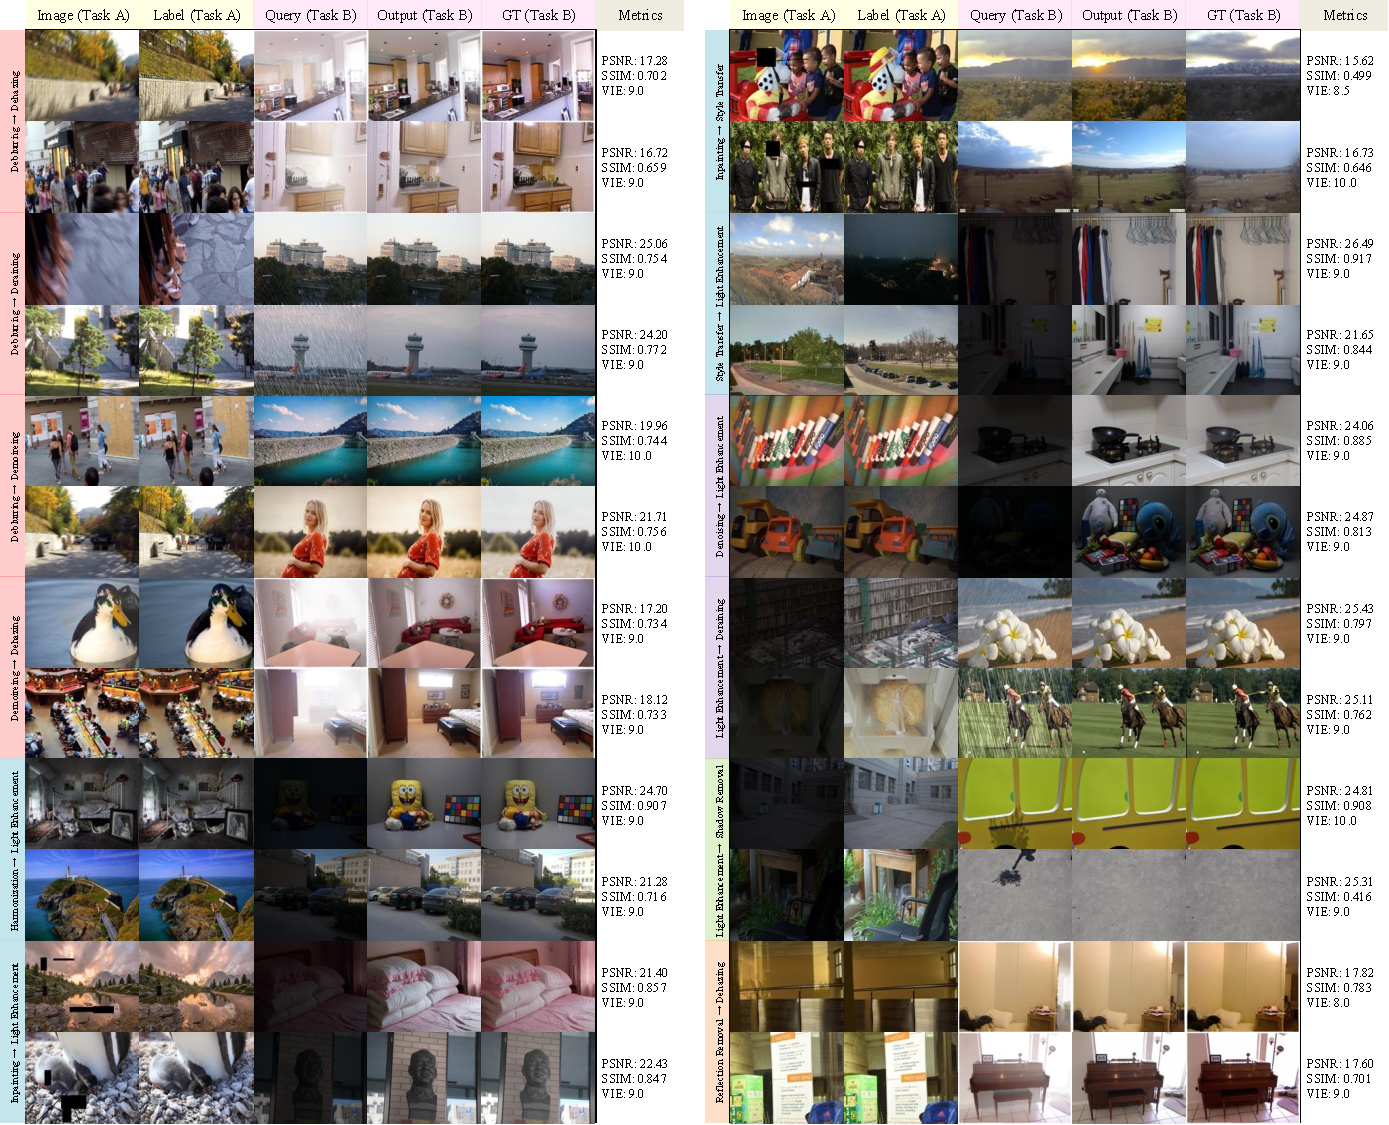
\includegraphics[width=\textwidth]{fig/figure4.pdf}
%     \caption{Representative Examples of Cross-Task In-Context Learning from Gemini in Twelve Pairs}
%     \label{fig:fig4}
% \vspace{-8pt}
% \end{figure*}

% \begin{figure*}[ht]
%     \centering
%     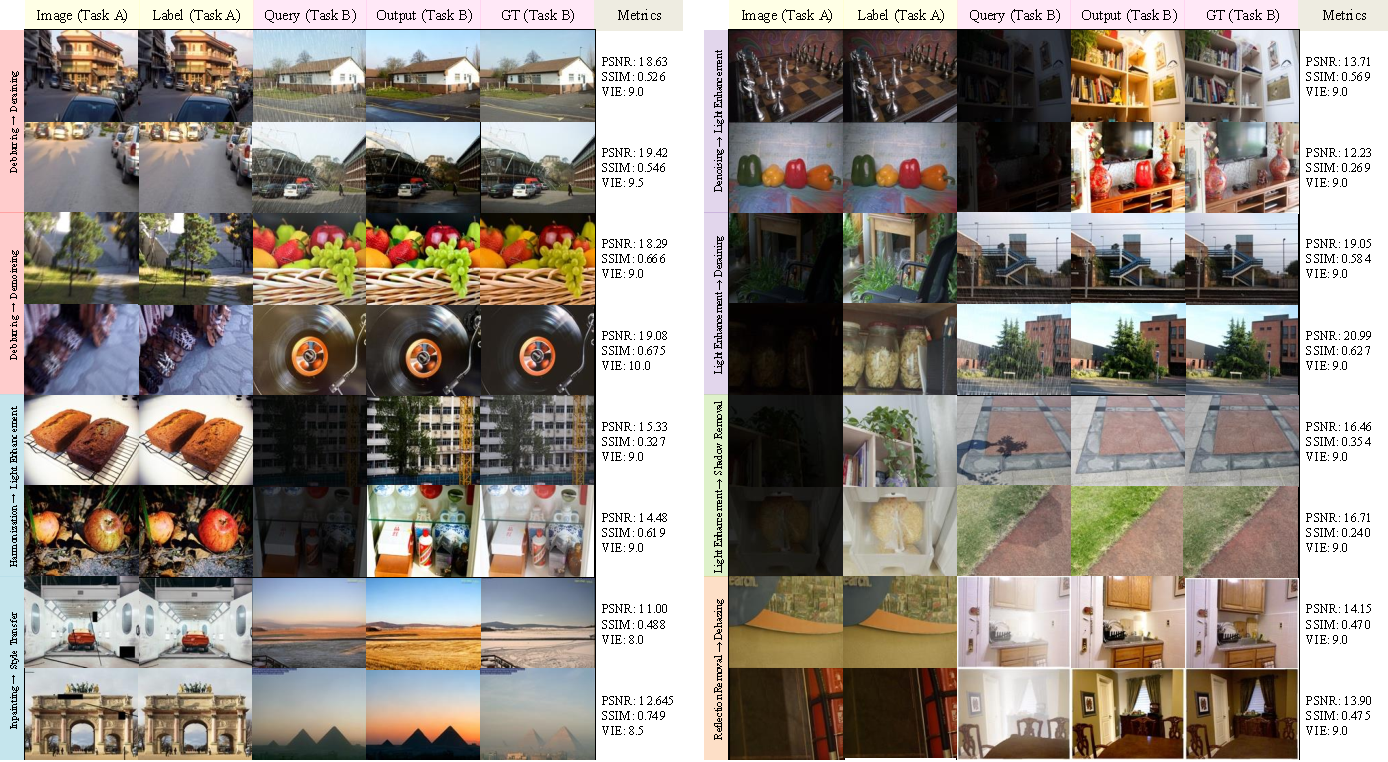
\includegraphics[width=\textwidth]{fig/figure6.pdf}
%     \caption{Representative Examples of Cross-Task In-Context Learning from Seedream in Eight Pairs}
%     \label{fig:fig6}
% \vspace{-8pt}
% \end{figure*}

% The Gemini (see Figure~\ref{fig:fig4}) and Seedream (see Figure~\ref{fig:fig6}) qualitative examples complement the quantitative results in the main paper. They use the same cross-task inference protocol: the fixed prompt and the Qwen-generated implicit prompt are applied to identical task-A demonstrations and task-B queries, while only the final image-editing backbone is changed. The figures illustrate representative examples of cross-task ICL, demonstrating how the VLM adapts flexibly to diverse tasks driven by conditioning implicit text prompts.

\subsection{Cross-Task Results of Seedream}
\label{sec:example}

\begin{figure*}[ht]
    \centering
    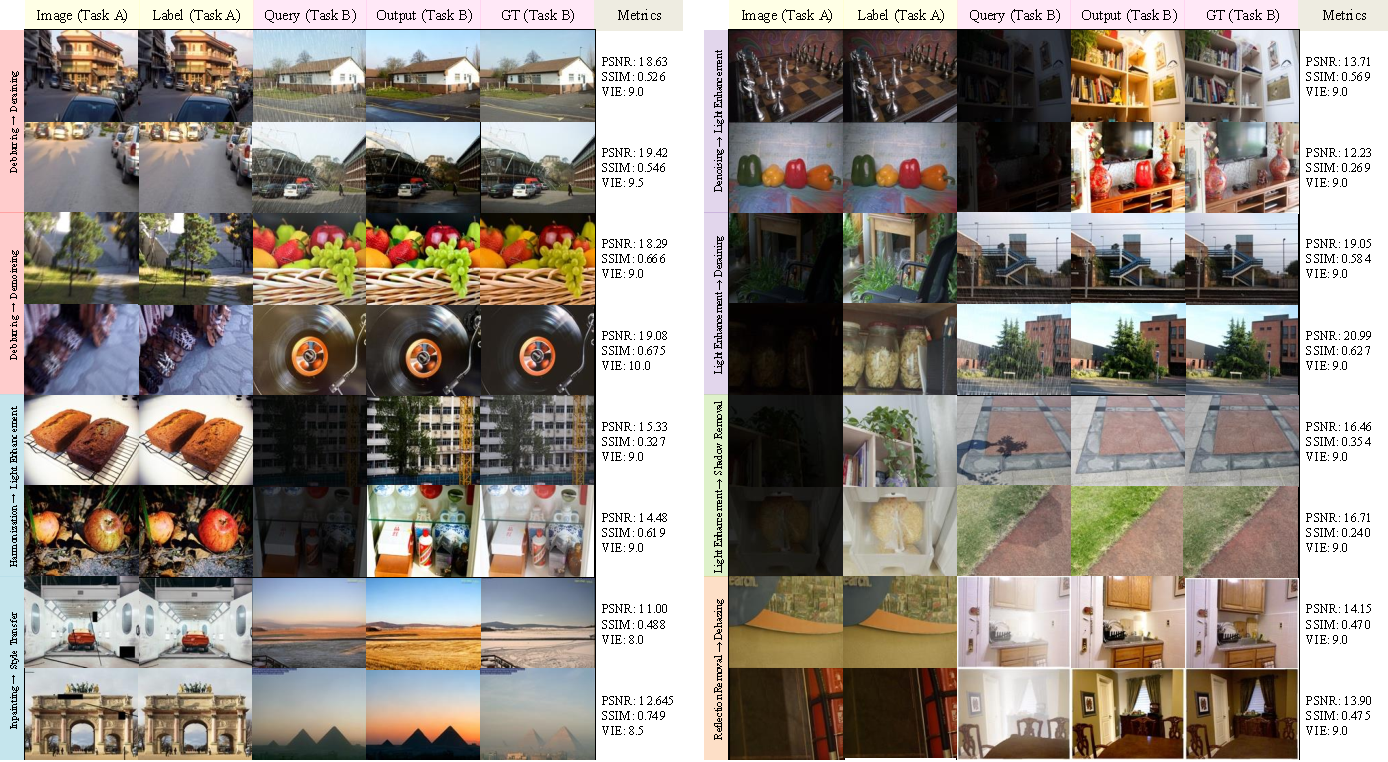
\includegraphics[width=\textwidth]{fig/figure6.pdf}
    \caption{Representative Examples of Cross-Task In-Context Learning from Seedream in Twelve Pairs}
    \label{fig:fig6}
\vspace{-8pt}
\end{figure*}

The Seedream qualitative examples complement the Gemini visual examples in the main paper. They use the same cross-task inference protocol: the fixed prompt and the Qwen-generated implicit prompt are applied to identical task-A demonstrations and task-B queries, while only the final image-editing backbone is changed. These cases are included to show that the qualitative gains of T2T-VICL are not specific to Gemini.


\subsection{Cross-Task Results of Other Models}
The generation ability of our pipeline to other image editing models is presented in Table~\ref{tab:5}. We further include additional open-source models for evaluation, including FLUX.2-dev~\cite{black2025flux}, OmniGen 2~\cite{wu2025omnigen2}, Qwen-Image-Edit~\cite{wu2025qwen, zhao2026qwen}, and FireRed~\cite{team2026firered}. This model choice stems from the VICL setting, in which VLMs accept multiple images and a textual prompt as input to generate a target image. At present, a limited number of any-to-any VLMs support this functionality. These selected VLMs are capable of handling multi-image inputs and generating edited images as outputs. Although different models may exhibit varying strengths across specific tasks, all evaluated models demonstrate a certain degree of cross-task generalization. In terms of overall performance, Gemini-2.5-Flash achieves the highest number of top-tier and second-tier cases across different task-transfer pairs. This observation further validates our choice of Gemini as the final image generation backbone in our framework.

% \begin{table*}[ht]
% \centering
% % \footnotesize
% \scriptsize
% \setlength{\tabcolsep}{0.6pt}
% \renewcommand{\arraystretch}{1.0}

% \captionsetup{width=0.96\textwidth, skip=4pt, type=table}
% \caption{Average of evaluation metrics, generated by baseline models (FLUX 2, OmniGen 2, Qwen-Image) with fixed prompts and Qwen prompts.}
% \vspace{-1pt}

% % \resizebox{\textwidth}{!}{
% \begin{adjustbox}{width=\textwidth}
% % \begin{tabular}{H *{6}{M} G *{6}{M} G *{6}{M}}
% \begin{tabular}{H *{18}{M}}
% \toprule
% \multirow{3}{*}{\textbf{Task}}
% & \multicolumn{6}{c}{\textbf{FLUX.2-dev}}
% & \multicolumn{6}{c}{\textbf{OmniGen 2}}
% & \multicolumn{6}{c}{\textbf{Qwen-Image-Edit}} \\
% % \cmidrule(lr){2-7} \cmidrule(lr){8-13} \cmidrule(lr){14-19}

% & \multicolumn{2}{c}{PSNR}
% & \multicolumn{2}{c}{SSIM}
% & \multicolumn{2}{c}{VIEScore}
% & \multicolumn{2}{c}{PSNR}
% & \multicolumn{2}{c}{SSIM}
% & \multicolumn{2}{c}{VIEScore}
% & \multicolumn{2}{c}{PSNR}
% & \multicolumn{2}{c}{SSIM}
% & \multicolumn{2}{c}{VIEScore} \\

% & \textcolor{gray}{Fix} & \textcolor{gray}{Ours}
% & \textcolor{gray}{Fix} & \textcolor{gray}{Ours}
% & \textcolor{gray}{Fix} & \textcolor{gray}{Ours}
% & \textcolor{gray}{Fix} & \textcolor{gray}{Ours}
% & \textcolor{gray}{Fix} & \textcolor{gray}{Ours}
% & \textcolor{gray}{Fix} & \textcolor{gray}{Ours}
% & \textcolor{gray}{Fix} & \textcolor{gray}{Ours}
% & \textcolor{gray}{Fix} & \textcolor{gray}{Ours}
% & \textcolor{gray}{Fix} & \textcolor{gray}{Ours} \\
% \midrule

% \rowcolor{lightred!30}
% \makecell[l]{Deblurring $\rightarrow$ Dehazing}
% & \cellcolor{lightred!60}8.53 & 8.50
% & 0.196 & \cellcolor{lightred!60}0.217
% & 2.61 & \cellcolor{lightred!60}3.88
% & 7.46 & \cellcolor{lightred!60}7.62
% & 0.175 & \cellcolor{lightred!60}0.183
% & 2.72 & \cellcolor{lightred!60}3.41
% & 8.16 & \cellcolor{lightred!60}8.56
% & 0.183 & \cellcolor{lightred!60}0.238
% & 3.58 & \cellcolor{lightred!60}5.73 \\
% \grayhline

% \rowcolor{lightred!30}
% \makecell[l]{Deblurring $\rightarrow$ Deraining}
% & 9.29 & \cellcolor{lightred!60}9.44
% & 0.160 & \cellcolor{lightred!60}0.162
% & 2.07 & \cellcolor{lightred!60}3.45
% & 8.22 & \cellcolor{lightred!60}8.22
% & \cellcolor{lightred!60}0.132 & 0.126
% & \cellcolor{lightred!60}2.64 & 2.17
% & 10.42 & \cellcolor{lightred!60}10.67
% & 0.188 & \cellcolor{lightred!60}0.234
% & 4.36 & \cellcolor{lightred!60}6.15 \\
% \grayhline

% \rowcolor{lightred!30}
% \makecell[l]{Dehazing $\rightarrow$ Denoising}
% & \cellcolor{lightred!60}8.81 & 8.70
% & \cellcolor{lightred!60}0.498 & 0.483
% & 4.68 & \cellcolor{lightred!60}4.77
% & 6.89 & \cellcolor{lightred!60}7.87
% & \cellcolor{lightred!60}0.404 & 0.403
% & 2.61 & \cellcolor{lightred!60}2.71
% & 11.91 & \cellcolor{lightred!60}15.61
% & 0.487 & \cellcolor{lightred!60}0.597
% & 3.71 & \cellcolor{lightred!60}6.10 \\
% \grayhline

% \rowcolor{lightred!30}
% \makecell[l]{Dehazing $\rightarrow$ Deraining}
% & \cellcolor{lightred!60}9.24 & 8.94
% & \cellcolor{lightred!60}0.207 & 0.205
% & 2.95 & \cellcolor{lightred!60}2.99
% & \cellcolor{lightred!60}7.49 & 7.08
% & \cellcolor{lightred!60}0.158 & 0.148
% & \cellcolor{lightred!60}2.19 & 2.13
% & 8.74 & \cellcolor{lightred!60}11.15
% & 0.177 & \cellcolor{lightred!60}0.276
% & 2.14 & \cellcolor{lightred!60}4.91 \\
% \grayhline

% \rowcolor{lightred!30}
% \makecell[l]{Denoising $\rightarrow$ Deblurring}
% & 10.07 & \cellcolor{lightred!60}10.12
% & \cellcolor{lightred!60}0.287 & 0.241
% & \cellcolor{lightred!60}6.38 & 6.08
% & 8.66 & \cellcolor{lightred!60}9.16
% & 0.273 & \cellcolor{lightred!60}0.280
% & 4.71 & \cellcolor{lightred!60}5.74
% & 9.59 & \cellcolor{lightred!60}10.36
% & 0.244 & \cellcolor{lightred!60}0.295
% & 4.63 & \cellcolor{lightred!60}7.33 \\
% \grayhline

% \rowcolor{lightblue!30}
% \makecell[l]{Colorization $\rightarrow$ Style Transfer}
% & \cellcolor{lightblue!60}9.72 & 8.42
% & \cellcolor{lightblue!60}0.302 & 0.250
% & 5.27 & \cellcolor{lightblue!60}6.42
% & \cellcolor{lightblue!60}7.89 & 7.42
% & \cellcolor{lightblue!60}0.248 & 0.211
% & \cellcolor{lightblue!60}4.13 & 3.44
% & \cellcolor{lightblue!60}9.24 & 9.10
% & 0.245 & \cellcolor{lightblue!60}0.279
% & 6.46 & \cellcolor{lightblue!60}6.54 \\
% \grayhline

% \rowcolor{lightblue!30}
% \makecell[l]{Harmonization $\rightarrow$ Light Enhancement}
% & \cellcolor{lightblue!60}9.09 & 8.32
% & \cellcolor{lightblue!60}0.222 & 0.180
% & \cellcolor{lightblue!60}7.77 & 7.55
% & \cellcolor{lightblue!60}8.32 & 7.34
% & \cellcolor{lightblue!60}0.202 & 0.143
% & 4.79 & \cellcolor{lightblue!60}5.59
% & \cellcolor{lightblue!60}9.32 & 8.85
% & \cellcolor{lightblue!60}0.277 & 0.230
% & 7.23 & \cellcolor{lightblue!60}8.18 \\
% \grayhline

% \rowcolor{lightblue!30}
% \makecell[l]{Inpainting $\rightarrow$ Harmonization}
% & 8.87 & \cellcolor{lightblue!60}9.48
% & 0.186 & \cellcolor{lightblue!60}0.203
% & 5.29 & \cellcolor{lightblue!60}6.39
% & \cellcolor{lightblue!60}7.91 & 7.79
% & \cellcolor{lightblue!60}0.176 & 0.165
% & \cellcolor{lightblue!60}3.32 & 3.16
% & \cellcolor{lightblue!60}10.42 & 10.08
% & \cellcolor{lightblue!60}0.263 & 0.260
% & 6.47 & \cellcolor{lightblue!60}7.09 \\
% \grayhline

% \rowcolor{lightblue!30}
% \makecell[l]{Inpainting $\rightarrow$ Style Transfer}
% & \cellcolor{lightblue!60}9.02 & 8.80
% & \cellcolor{lightblue!60}0.201 & 0.189
% & 2.26 & \cellcolor{lightblue!60}3.78
% & \cellcolor{lightblue!60}8.30 & 7.76
% & \cellcolor{lightblue!60}0.208 & 0.185
% & 3.87 & \cellcolor{lightblue!60}4.10
% & \cellcolor{lightblue!60}9.12 & 9.09
% & 0.207 & \cellcolor{lightblue!60}0.231
% & 4.40 & \cellcolor{lightblue!60}5.00 \\
% \grayhline

% \rowcolor{lightblue!30}
% \makecell[l]{Style Transfer $\rightarrow$ Light Enhancement}
% & \cellcolor{lightblue!60}9.58 & 8.59
% & \cellcolor{lightblue!60}0.289 & 0.245
% & \cellcolor{lightblue!60}6.14 & 6.00
% & \cellcolor{lightblue!60}8.35 & 7.92
% & \cellcolor{lightblue!60}0.232 & 0.186
% & 2.30 & \cellcolor{lightblue!60}3.53
% & \cellcolor{lightblue!60}10.19 & 9.64
% & \cellcolor{lightblue!60}0.318 & 0.281
% & 5.24 & \cellcolor{lightblue!60}6.28 \\
% \grayhline

% \rowcolor{lightyellow!30}
% \makecell[l]{Shadow Removal $\rightarrow$ Reflection Removal}
% & 8.08 & \cellcolor{lightyellow!60}11.73
% & 0.251 & \cellcolor{lightyellow!60}0.344
% & 2.79 & \cellcolor{lightyellow!60}5.37
% & 8.45 & \cellcolor{lightyellow!60}8.99
% & \cellcolor{lightyellow!60}0.226 & 0.215
% & 2.60 & \cellcolor{lightyellow!60}3.16
% & 9.09 & \cellcolor{lightyellow!60}10.78
% & 0.161 & \cellcolor{lightyellow!60}0.318
% & 3.06 & \cellcolor{lightyellow!60}3.93 \\
% \grayhline

% \rowcolor{lightpurple!30}
% \makecell[l]{Denoising $\rightarrow$ Light Enhancement}
% & \cellcolor{lightpurple!60}9.63 & 8.56
% & \cellcolor{lightpurple!60}0.260 & 0.193
% & 7.12 & \cellcolor{lightpurple!60}7.62
% & \cellcolor{lightpurple!60}8.57 & 7.50
% & \cellcolor{lightpurple!60}0.218 & 0.146
% & 6.62 & \cellcolor{lightpurple!60}7.08
% & \cellcolor{lightpurple!60}9.09 & 7.99
% & \cellcolor{lightpurple!60}0.252 & 0.183
% & 5.83 & \cellcolor{lightpurple!60}6.76 \\
% \grayhline

% \rowcolor{lightorange!30}
% \makecell[l]{Reflection Removal $\rightarrow$ Dehazing}
% & 8.77 & \cellcolor{lightorange!50}9.45
% & 0.276 & \cellcolor{lightorange!50}0.308
% & 4.49 & \cellcolor{lightorange!50}5.88
% & \cellcolor{lightorange!50}7.40 & 7.30
% & \cellcolor{lightorange!50}0.241 & 0.236
% & 4.12 & \cellcolor{lightorange!50}4.88
% & \cellcolor{lightorange!50}8.55 & 8.46
% & 0.251 & \cellcolor{lightorange!50}0.270
% & 4.11 & \cellcolor{lightorange!50}6.19 \\
% \grayhline

% \rowcolor{lightorange!30}
% \makecell[l]{Shadow Removal $\rightarrow$ Deraining}
% & 9.00 & \cellcolor{lightorange!50}11.80
% & 0.230 & \cellcolor{lightorange!50}0.261
% & 2.67 & \cellcolor{lightorange!50}4.44
% & 8.02 & \cellcolor{lightorange!50}8.48
% & \cellcolor{lightorange!50}0.146 & 0.134
% & 2.00 & \cellcolor{lightorange!50}2.71
% & 9.89 & \cellcolor{lightorange!50}10.44
% & 0.165 & \cellcolor{lightorange!50}0.213
% & 3.71 & \cellcolor{lightorange!50}3.71 \\

% \bottomrule
% \end{tabular} % }
% \end{adjustbox}
% \end{table*}



\begin{table*}[ht]
\centering
\scriptsize
\setlength{\tabcolsep}{0.5pt}
\renewcommand{\arraystretch}{0.88}
\captionsetup{width=0.98\textwidth, skip=4pt, type=table}
\caption{Average of evaluation metrics for additional backbones, generated by open-source models (FLUX 2, OmniGen 2, Qwen-Image, and FireRed) with fixed prompts and Qwen prompts.}
\vspace{-2pt}
\label{tab:5}

% ---------- (a) ----------
\begin{subtable}[t]{\textwidth}
\centering
\caption{FLUX.2-dev and OmniGen 2}
\vspace{-3pt}
\begin{adjustbox}{width=\textwidth}
\begin{tabular}{>{\raggedright\arraybackslash}m{4cm} *{5}{>{\centering\arraybackslash}m{0.8cm}} >{\centering\arraybackslash}m{1cm} *{5}{>{\centering\arraybackslash}m{0.8cm}} >{\centering\arraybackslash}m{1cm}}
\toprule
\multirow{3}{*}{\textbf{Task}}
& \multicolumn{6}{c}{\textbf{FLUX.2-dev}}
& \multicolumn{6}{c}{\textbf{OmniGen 2}} \\
& \multicolumn{2}{c}{\textbf{PSNR}$\uparrow$}
& \multicolumn{2}{c}{\textbf{SSIM}$\uparrow$}
& \multicolumn{2}{c}{\textbf{VIEScore}$\uparrow$}
& \multicolumn{2}{c}{\textbf{PSNR}$\uparrow$}
& \multicolumn{2}{c}{\textbf{SSIM}$\uparrow$}
& \multicolumn{2}{c}{\textbf{VIEScore}$\uparrow$} \\
& \textcolor{gray}{\textbf{Fixed}} & \textcolor{gray}{\textbf{Ours}}
& \textcolor{gray}{\textbf{Fixed}} & \textcolor{gray}{\textbf{Ours}}
& \textcolor{gray}{\textbf{Fixed}} & \textcolor{gray}{\textbf{Ours}}
& \textcolor{gray}{\textbf{Fixed}} & \textcolor{gray}{\textbf{Ours}}
& \textcolor{gray}{\textbf{Fixed}} & \textcolor{gray}{\textbf{Ours}}
& \textcolor{gray}{\textbf{Fixed}} & \textcolor{gray}{\textbf{Ours}} \\
\midrule
\rowcolor{lightred!30}
Deblurring $\rightarrow$ Dehazing
& \cellcolor{lightred!60}8.53 & 8.50
& 0.196 & \cellcolor{lightred!60}0.217
& 2.61 & \cellcolor{lightred!60}\tabgainsubscript{3.88}{+1.27}
& 7.46 & \cellcolor{lightred!60}7.62
& 0.175 & \cellcolor{lightred!60}0.183
& 2.72 & \cellcolor{lightred!60}\tabgainsubscript{3.41}{+0.69} \\
\grayhline
\rowcolor{lightred!30}
Dehazing $\rightarrow$ Denoising
& \cellcolor{lightred!60}8.81 & 8.70
& \cellcolor{lightred!60}0.498 & 0.483
& 4.68 & \cellcolor{lightred!60}\tabgainsubscript{4.77}{+0.09}
& 6.89 & \cellcolor{lightred!60}7.87
& \cellcolor{lightred!60}0.404 & 0.403
& 2.61 & \cellcolor{lightred!60}\tabgainsubscript{2.71}{+0.10} \\
\grayhline
\rowcolor{lightred!30}
Deraining $\rightarrow$ Demoireing
& \cellcolor{lightred!60}9.51 & 8.99
& \cellcolor{lightred!60}0.461 & 0.444
& \cellcolor{lightred!60}5.05 & \tablosssubscript{5.03}{-0.02}
& 7.40 & \cellcolor{lightred!60}7.55
& 0.373 & \cellcolor{lightred!60}0.375
& 2.66 & \cellcolor{lightred!60}\tabgainsubscript{2.98}{+0.32} \\
\grayhline
\rowcolor{lightblue!30}
Harmonization $\rightarrow$ Style Transfer
& \cellcolor{lightblue!60}9.07 & 8.83
& \cellcolor{lightblue!60}0.253 & 0.246
& 2.95 & \cellcolor{lightblue!60}\tabgainsubscript{5.68}{+2.73}
& \cellcolor{lightblue!60}8.44 & 7.84
& \cellcolor{lightblue!60}0.251 & 0.227
& 5.03 & \cellcolor{lightblue!60}\tabsamesubscript{5.03}{+0.00} \\
\grayhline
\rowcolor{lightblue!30}
Inpainting $\rightarrow$ Style Transfer
& \cellcolor{lightblue!60}9.02 & 8.80
& \cellcolor{lightblue!60}0.201 & 0.189
& 2.26 & \cellcolor{lightblue!60}\tabgainsubscript{3.78}{+1.52}
& \cellcolor{lightblue!60}8.30 & 7.76
& \cellcolor{lightblue!60}0.208 & 0.185
& 3.87 & \cellcolor{lightblue!60}\tabgainsubscript{4.10}{+0.23} \\
\grayhline
\rowcolor{lightyellow!30}
Shadow Removal $\rightarrow$ Reflection Removal
& 8.08 & \cellcolor{lightyellow!60}11.73
& 0.251 & \cellcolor{lightyellow!60}0.344
& 2.79 & \cellcolor{lightyellow!60}\tabgainsubscript{5.37}{+2.58}
& 8.45 & \cellcolor{lightyellow!60}8.99
& \cellcolor{lightyellow!60}0.226 & 0.215
& 2.60 & \cellcolor{lightyellow!60}\tabgainsubscript{3.16}{+0.56} \\
\grayhline
\rowcolor{lightpurple!30}
Denoising $\rightarrow$ Light Enhancement
& \cellcolor{lightpurple!60}9.63 & 8.56
& \cellcolor{lightpurple!60}0.260 & 0.193
& 7.12 & \cellcolor{lightpurple!60}\tabgainsubscript{7.62}{+0.50}
& \cellcolor{lightpurple!60}8.57 & 7.50
& \cellcolor{lightpurple!60}0.218 & 0.146
& 6.62 & \cellcolor{lightpurple!60}\tabgainsubscript{7.08}{+0.46} \\
\grayhline
\rowcolor{lightorange!30}
Reflection Removal $\rightarrow$ Dehazing
& 8.77 & \cellcolor{lightorange!50}9.45
& 0.276 & \cellcolor{lightorange!50}0.308
& 4.49 & \cellcolor{lightorange!50}\tabgainsubscript{5.88}{+1.39}
& \cellcolor{lightorange!50}7.40 & 7.30
& \cellcolor{lightorange!50}0.241 & 0.236
& 4.12 & \cellcolor{lightorange!50}\tabgainsubscript{4.88}{+0.76} \\
\grayhline
\rowcolor{lightorange!30}
Shadow Removal $\rightarrow$ Deraining
& 9.00 & \cellcolor{lightorange!50}11.80
& 0.230 & \cellcolor{lightorange!50}0.261
& 2.67 & \cellcolor{lightorange!50}\tabgainsubscript{4.44}{+1.77}
& 8.02 & \cellcolor{lightorange!50}8.48
& \cellcolor{lightorange!50}0.146 & 0.134
& 2.00 & \cellcolor{lightorange!50}\tabgainsubscript{2.71}{+0.71} \\
\bottomrule
\end{tabular}
\end{adjustbox}
\end{subtable}

\vspace{3pt}

\begin{subtable}[t]{\textwidth}
\centering
\caption{Qwen-Image-Edit-2511 and FireRed-Image-Edit-1.1}
\vspace{-3pt}
\begin{adjustbox}{width=\textwidth}
\begin{tabular}{>{\raggedright\arraybackslash}m{4cm} *{5}{>{\centering\arraybackslash}m{0.8cm}} >{\centering\arraybackslash}m{1cm} *{5}{>{\centering\arraybackslash}m{0.8cm}} >{\centering\arraybackslash}m{1cm}}
\toprule
\multirow{3}{*}{\textbf{Task}}
& \multicolumn{6}{c}{\textbf{Qwen-Image-Edit}}
& \multicolumn{6}{c}{\textbf{FireRed-Image-Edit}} \\
& \multicolumn{2}{c}{\textbf{PSNR}$\uparrow$}
& \multicolumn{2}{c}{\textbf{SSIM}$\uparrow$}
& \multicolumn{2}{c}{\textbf{VIEScore}$\uparrow$}
& \multicolumn{2}{c}{\textbf{PSNR}$\uparrow$}
& \multicolumn{2}{c}{\textbf{SSIM}$\uparrow$}
& \multicolumn{2}{c}{\textbf{VIEScore}$\uparrow$} \\
& \textcolor{gray}{\textbf{Fixed}} & \textcolor{gray}{\textbf{Ours}}
& \textcolor{gray}{\textbf{Fixed}} & \textcolor{gray}{\textbf{Ours}}
& \textcolor{gray}{\textbf{Fixed}} & \textcolor{gray}{\textbf{Ours}}
& \textcolor{gray}{\textbf{Fixed}} & \textcolor{gray}{\textbf{Ours}}
& \textcolor{gray}{\textbf{Fixed}} & \textcolor{gray}{\textbf{Ours}}
& \textcolor{gray}{\textbf{Fixed}} & \textcolor{gray}{\textbf{Ours}} \\
\midrule
\rowcolor{lightred!30}
Deblurring $\rightarrow$ Dehazing
& 8.16 & \cellcolor{lightred!60}8.56
& 0.183 & \cellcolor{lightred!60}0.238
& 3.58 & \cellcolor{lightred!60}\tabgainsubscript{5.73}{+2.15}
& \cellcolor{lightred!60}8.90 & 8.27
& \cellcolor{lightred!60}0.260 & 0.178
& 6.16 & \cellcolor{lightred!60}\tabgainsubscript{6.46}{+0.30} \\
\grayhline
\rowcolor{lightred!30}
Deblurring $\rightarrow$ Deraining
& 10.42 & \cellcolor{lightred!60}10.67
& 0.188 & \cellcolor{lightred!60}0.234
& 4.36 & \cellcolor{lightred!60}\tabgainsubscript{6.15}{+1.79}
& \cellcolor{lightred!60}9.35 & 8.92
& \cellcolor{lightred!60}0.164 & 0.139
& 5.20 & \cellcolor{lightred!60}\tabgainsubscript{6.21}{+1.01} \\
\grayhline
\rowcolor{lightred!30}
Dehazing $\rightarrow$ Denoising
& 11.91 & \cellcolor{lightred!60}15.61
& 0.487 & \cellcolor{lightred!60}0.597
& 3.71 & \cellcolor{lightred!60}\tabgainsubscript{6.10}{+2.39}
& 7.87 & \cellcolor{lightred!60}9.09
& 0.457 & \cellcolor{lightred!60}0.473
& 5.78 & \cellcolor{lightred!60}\tabgainsubscript{6.03}{+0.25} \\
\grayhline
\rowcolor{lightred!30}
Dehazing $\rightarrow$ Deraining
& 8.74 & \cellcolor{lightred!60}11.15
& 0.177 & \cellcolor{lightred!60}0.276
& 2.14 & \cellcolor{lightred!60}\tabgainsubscript{4.91}{+2.77}
& 8.56 & \cellcolor{lightred!60}8.68
& \cellcolor{lightred!60}0.193 & 0.181
& 3.08 & \cellcolor{lightred!60}\tabgainsubscript{3.94}{+0.86} \\
\grayhline
\rowcolor{lightred!30}
Demoireing $\rightarrow$ Dehazing
& 8.54 & \cellcolor{lightred!60}8.57
& 0.229 & \cellcolor{lightred!60}0.271
& 4.07 & \cellcolor{lightred!60}\tabgainsubscript{5.31}{+1.24}
& 8.71 & \cellcolor{lightred!60}9.23
& 0.276 & \cellcolor{lightred!60}0.294
& 5.41 & \cellcolor{lightred!60}\tabgainsubscript{6.16}{+0.75} \\
\grayhline
\rowcolor{lightred!30}
Denoising $\rightarrow$ Deblurring
& 9.59 & \cellcolor{lightred!60}10.36
& 0.244 & \cellcolor{lightred!60}0.295
& 4.63 & \cellcolor{lightred!60}\tabgainsubscript{7.33}{+2.70}
& 9.72 & \cellcolor{lightred!60}9.99
& 0.263 & \cellcolor{lightred!60}0.293
& 7.13 & \cellcolor{lightred!60}\tabgainsubscript{8.49}{+1.36} \\
\grayhline
\rowcolor{lightblue!30}
Colorization $\rightarrow$ Style Transfer
& \cellcolor{lightblue!60}9.24 & 9.10
& 0.245 & \cellcolor{lightblue!60}0.279
& 6.46 & \cellcolor{lightblue!60}\tabgainsubscript{6.54}{+0.08}
& \cellcolor{lightblue!60}8.75 & 8.46
& \cellcolor{lightblue!60}0.262 & 0.235
& 7.10 & \cellcolor{lightblue!60}\tabgainsubscript{7.90}{+0.80} \\
\grayhline
\rowcolor{lightblue!30}
Harmonization $\rightarrow$ Light Enhancement
& \cellcolor{lightblue!60}9.32 & 8.85
& \cellcolor{lightblue!60}0.277 & 0.230
& 7.23 & \cellcolor{lightblue!60}\tabgainsubscript{8.18}{+0.95}
& \cellcolor{lightblue!60}8.97 & 8.77
& \cellcolor{lightblue!60}0.225 & 0.205
& 8.14 & \cellcolor{lightblue!60}\tabgainsubscript{8.33}{+0.19} \\
\grayhline
\rowcolor{lightblue!30}
Inpainting $\rightarrow$ Style Transfer
& \cellcolor{lightblue!60}9.12 & 9.09
& 0.207 & \cellcolor{lightblue!60}0.231
& 4.40 & \cellcolor{lightblue!60}\tabgainsubscript{5.00}{+0.60}
& \cellcolor{lightblue!60}9.08 & 8.82
& \cellcolor{lightblue!60}0.211 & 0.198
& 4.12 & \cellcolor{lightblue!60}\tabgainsubscript{5.08}{+0.96} \\
\grayhline
\rowcolor{lightyellow!30}
Shadow Removal $\rightarrow$ Reflection Removal
& 9.09 & \cellcolor{lightyellow!60}10.78
& 0.161 & \cellcolor{lightyellow!60}0.318
& 3.06 & \cellcolor{lightyellow!60}\tabgainsubscript{3.93}{+0.87}
& \cellcolor{lightyellow!60}9.11 & 8.43
& \cellcolor{lightyellow!60}0.226 & 0.210
& 3.35 & \cellcolor{lightyellow!60}\tabgainsubscript{3.55}{+0.20} \\
\grayhline
\rowcolor{lightpurple!30}
Denoising $\rightarrow$ Light Enhancement
& \cellcolor{lightpurple!60}9.09 & 7.99
& \cellcolor{lightpurple!60}0.252 & 0.183
& 5.83 & \cellcolor{lightpurple!60}\tabgainsubscript{6.76}{+0.93}
& \cellcolor{lightpurple!60}9.60 & 9.22
& \cellcolor{lightpurple!60}0.254 & 0.224
& 8.64 & \cellcolor{lightpurple!60}\tabgainsubscript{8.70}{+0.06} \\
\grayhline
\rowcolor{lightpurple!30}
Light Enhancement $\rightarrow$ Deraining
& 9.51 & \cellcolor{lightpurple!60}10.07
& 0.203 & \cellcolor{lightpurple!60}0.231
& 3.47 & \cellcolor{lightpurple!60}\tabgainsubscript{3.48}{+0.01}
& \cellcolor{lightpurple!60}9.08 & 8.80
& \cellcolor{lightpurple!60}0.191 & 0.177
& 5.23 & \cellcolor{lightpurple!60}\tabgainsubscript{5.41}{+0.18} \\
\grayhline
\rowcolor{lightorange!30}
Reflection Removal $\rightarrow$ Dehazing
& \cellcolor{lightorange!50}8.55 & 8.46
& 0.251 & \cellcolor{lightorange!50}0.270
& 4.11 & \cellcolor{lightorange!50}\tabgainsubscript{6.19}{+2.08}
& \cellcolor{lightorange!50}8.53 & 8.18
& \cellcolor{lightorange!50}0.277 & 0.240
& 6.50 & \cellcolor{lightorange!50}\tabgainsubscript{7.55}{+1.05} \\
\grayhline
\rowcolor{lightorange!30}
Shadow Removal $\rightarrow$ Deraining
& 9.89 & \cellcolor{lightorange!50}10.44
& 0.165 & \cellcolor{lightorange!50}0.213
& 3.71 & \cellcolor{lightorange!50}\tabsamesubscript{3.71}{+0.00}
& \cellcolor{lightorange!50}10.01 & 8.87
& \cellcolor{lightorange!50}0.191 & 0.173
& 3.85 & \cellcolor{lightorange!50}\tabgainsubscript{4.07}{+0.22} \\
\bottomrule
\end{tabular}
\end{adjustbox}
\end{subtable}

\vspace{-6pt}
\end{table*}



\subsection{Second-Tier Typed Result Explanation}
\label{sec:viescore}

The second-tier group contains task pairs where T2T-VICL consistently improves VIEScore, while PSNR or SSIM may decrease. We may not interpret these cases as failures of cross-task VICL, as the visual consistency of most generated results remains comparable to those in the top-tier group (see Figure~\ref{fig:fig5}). The gap instead might indicate a mismatch between pixel-aligned fidelity metrics and the goal of several specific target tasks, especially when the target task is closer to conditional generation than deterministic restoration. This issue is especially clear for colorization and style transfer, which have inherent one-to-many ambiguity: multiple plausible outputs may correspond to the same input~\cite{su2020instance,kang2023ddcolor}.

\begin{figure*}[ht]
    \centering
    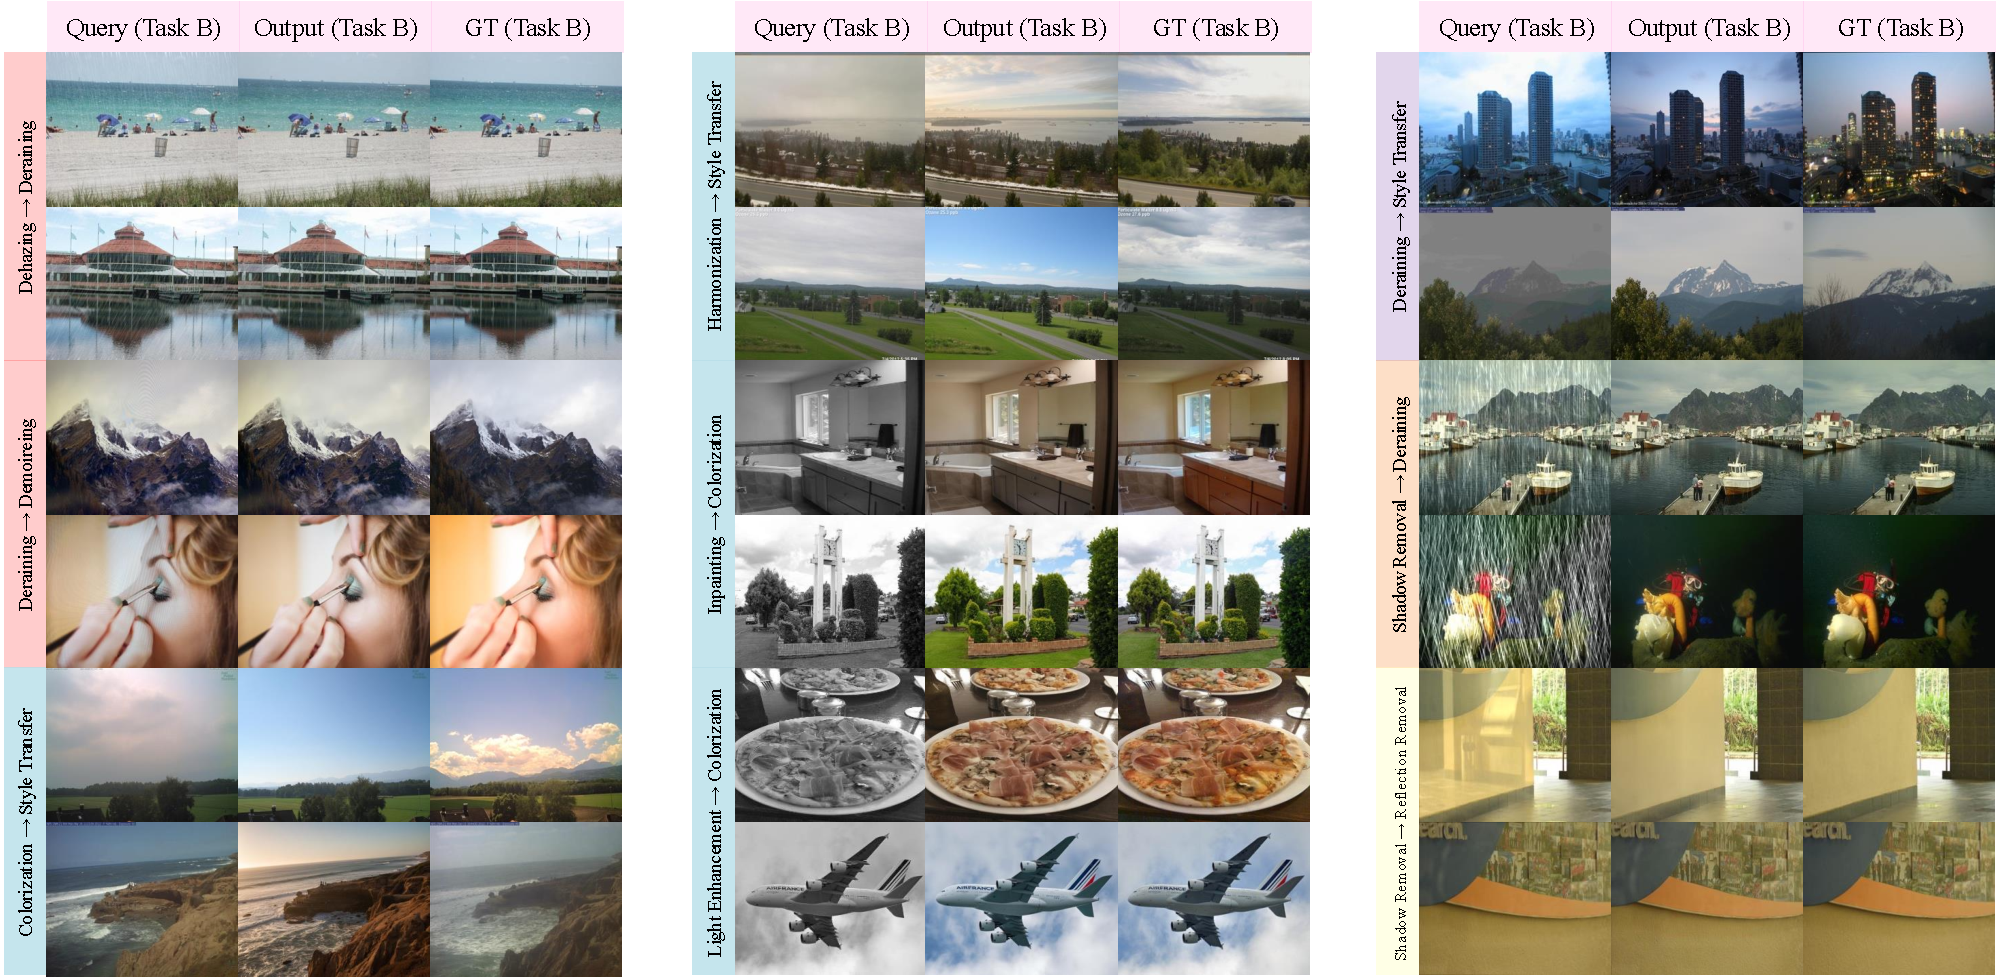
\includegraphics[width=\textwidth]{fig/figure5.pdf}
    \caption{Representative Examples of Cross-Task In-Context Learning from Gemini in Nine Pairs}
    \label{fig:fig5}
\vspace{-8pt}
\end{figure*}

In colorization, an output that remains close to the grayscale input can preserve luminance structure and obtain competitive PSNR or SSIM, even if it fails to add plausible chroma. Recent colorization studies still commonly report PSNR and SSIM, but they increasingly supplement them with perceptual, distributional, or color-statistical measures such as LPIPS, FID, and colorfulness-related metrics~\cite{wu2021towards,kang2023ddcolor}. This is not because PSNR/SSIM are invalid, but because pixel-level fidelity alone cannot fully capture color plausibility under a one-to-many target distribution. A VIEScore improvement with a small PSNR/SSIM drop can therefore still correspond to better task performance.

Style transfer has an even weaker one-to-one correspondence assumption: a successful stylized image should preserve semantic content while intentionally changing appearance, texture, and color statistics. Accordingly, style-transfer studies often report perceptual measures and human preference evaluation rather than solely PSNR or SSIM metrics~\cite{deng2022stytr2, wright2022artfid}.

These related observations actually support our use of VIEScore as the primary signal for the second-tier group, because VIEScore is able to evaluate whether the output follows the intended visual instruction and preserves the relevant content. The consistent superiority of VIEScore over IQA metrics in the second-tier group suggests that our approach prioritizes semantic preservation and cross-task coherence.

To complement the PSNR/SSIM-based analysis, we evaluate all task pairs whose target task is colorization, style transfer, or deraining using perceptual, distributional, and color-aware metrics. Table~\ref{tab:new-metrics} reports Fixed and Ours side by side for each backbone; lower values indicate better agreement with the task-B ground truth or target distribution. CIEDE2000 is used only for colorization/style-transfer targets, ArtFID only for style-transfer targets, and deraining-target rows are evaluated with LPIPS, DISTS, and FID.

\begin{table*}[t]
\centering
\scriptsize
\setlength{\tabcolsep}{2.8pt}
\caption{Additional evaluation metrics for targeted task pairs. All metrics are lower-is-better; within each Fixed/Ours pair, the lower value is shown in bold. CIEDE2000 is reported only for target tasks involving colorization or style transfer, and ArtFID is reported only when the target task is style transfer.}
\label{tab:new-metrics}
\resizebox{\textwidth}{!}{%
\begin{tabular}{lcccccccccc}
\toprule
\multicolumn{11}{c}{\textbf{Gemini 2.5 Flash}} \\
\midrule
\multirow{2}{*}{Task Pair} & \multicolumn{2}{c}{CIEDE$\downarrow$} & \multicolumn{2}{c}{LPIPS$\downarrow$} & \multicolumn{2}{c}{DISTS$\downarrow$} & \multicolumn{2}{c}{FID$\downarrow$} & \multicolumn{2}{c}{ArtFID$\downarrow$} \\
\cmidrule(lr){2-3}\cmidrule(lr){4-5}\cmidrule(lr){6-7}\cmidrule(lr){8-9}\cmidrule(lr){10-11}
 & Fixed & Ours & Fixed & Ours & Fixed & Ours & Fixed & Ours & Fixed & Ours \\
\midrule
Deblurring $\rightarrow$ Deraining & -- & -- & 0.226 & \textbf{0.194} & 0.158 & \textbf{0.138} & 79.3 & \textbf{63.3} & -- & -- \\
Dehazing $\rightarrow$ Deraining & -- & -- & 0.219 & \textbf{0.204} & 0.150 & \textbf{0.139} & 80.3 & \textbf{73.6} & -- & -- \\
Colorization $\rightarrow$ Style Transfer & \textbf{18.56} & 19.81 & 0.522 & \textbf{0.520} & 0.242 & \textbf{0.239} & 98.5 & \textbf{97.5} & \textbf{100.2} & 102.4 \\
Harmonization $\rightarrow$ Style Transfer & \textbf{19.00} & 19.50 & 0.550 & \textbf{0.530} & 0.264 & \textbf{0.246} & 117.5 & \textbf{102.4} & 105.8 & \textbf{100.1} \\
Inpainting $\rightarrow$ Colorization & 10.63 & \textbf{10.60} & 0.247 & \textbf{0.209} & 0.165 & \textbf{0.144} & 97.9 & \textbf{80.8} & -- & -- \\
Inpainting $\rightarrow$ Style Transfer & 28.87 & \textbf{19.23} & 0.796 & \textbf{0.508} & 0.443 & \textbf{0.236} & 274.4 & \textbf{99.3} & 284.5 & \textbf{98.3} \\
Light Enhancement $\rightarrow$ Colorization & \textbf{9.83} & 10.24 & 0.219 & \textbf{0.206} & 0.152 & \textbf{0.141} & 91.8 & \textbf{78.4} & -- & -- \\
Deraining $\rightarrow$ Style Transfer & \textbf{18.44} & 19.18 & 0.574 & \textbf{0.524} & 0.269 & \textbf{0.236} & 121.2 & \textbf{99.8} & 126.0 & \textbf{103.9} \\
Light Enhancement $\rightarrow$ Deraining & -- & -- & 0.274 & \textbf{0.179} & 0.189 & \textbf{0.127} & 109.0 & \textbf{58.2} & -- & -- \\
Shadow Removal $\rightarrow$ Deraining & -- & -- & 0.202 & \textbf{0.198} & 0.143 & \textbf{0.139} & 69.3 & \textbf{64.7} & -- & -- \\
\bottomrule
\end{tabular}%
}
\vspace{0.6em}
\resizebox{\textwidth}{!}{%
\begin{tabular}{lcccccccccc}
\toprule
\multicolumn{11}{c}{\textbf{Seedream 4.0}} \\
\midrule
\multirow{2}{*}{Task Pair} & \multicolumn{2}{c}{CIEDE$\downarrow$} & \multicolumn{2}{c}{LPIPS$\downarrow$} & \multicolumn{2}{c}{DISTS$\downarrow$} & \multicolumn{2}{c}{FID$\downarrow$} & \multicolumn{2}{c}{ArtFID$\downarrow$} \\
\cmidrule(lr){2-3}\cmidrule(lr){4-5}\cmidrule(lr){6-7}\cmidrule(lr){8-9}\cmidrule(lr){10-11}
 & Fixed & Ours & Fixed & Ours & Fixed & Ours & Fixed & Ours & Fixed & Ours \\
\midrule
Deblurring $\rightarrow$ Deraining & -- & -- & 0.414 & \textbf{0.398} & 0.250 & \textbf{0.239} & 135.9 & \textbf{113.8} & -- & -- \\
Dehazing $\rightarrow$ Deraining & -- & -- & 0.371 & \textbf{0.357} & \textbf{0.228} & 0.229 & 119.2 & \textbf{112.5} & -- & -- \\
Colorization $\rightarrow$ Style Transfer & \textbf{28.40} & 29.21 & 0.629 & \textbf{0.623} & 0.297 & \textbf{0.295} & 113.2 & \textbf{103.0} & 139.1 & \textbf{132.5} \\
Light Enhancement $\rightarrow$ Colorization & 23.39 & \textbf{22.82} & 0.412 & \textbf{0.383} & 0.223 & \textbf{0.208} & 130.3 & \textbf{103.7} & -- & -- \\
Light Enhancement $\rightarrow$ Deraining & -- & -- & 0.398 & \textbf{0.364} & 0.255 & \textbf{0.228} & 131.6 & \textbf{104.4} & -- & -- \\
\bottomrule
\end{tabular}%
}
\end{table*}


\end{document}
